\chapter*{ECRICOME 2017 : le corrigé}
  
%

\section*{Exercice 1}

\noindent
Dans tout l'exercice, on notera $\M{3}$ l'ensemble des matrices
carrées d'ordre $3$ et $I$ la matrice identité d'ordre $3$. On
considère la matrice $a$ définie par :
\[
A = 
\begin{smatrix}
  0 & 1 & 2\\
  -1 & 2 & 2\\
  -3 & 3 & 1
\end{smatrix}
\]

\subsection*{Partie A : Étude de la matrice $A$}
\begin{noliste}{1.}
\item Calculer les matrices $(A-I)^2$ et $(A-I)^3$.

\begin{proof}~
\[
 (A-I)^2 = 
 \begin{smatrix}
  -1 & 1 & 2\\ 
  -1 & 1 & 2\\ 
  -3 & 3 & 0
 \end{smatrix}
 \begin{smatrix}
  -1 & 1 & 2\\ 
  -1 & 1 & 2\\ 
  -3 & 3 & 0
 \end{smatrix}
 = 
 \begin{smatrix} 
 -6 & 6 & 0\\ 
 -6 & 6 & 0\\ 
 0 & 0 & 0
 \end{smatrix}
\]
\[
 (A-I)^3 = (A-I)(A-I)^2 =
 \begin{smatrix}
  -1 & 1 & 2\\ 
  -1 & 1 & 2\\ 
  -3 & 3 & 0
 \end{smatrix}
 \begin{smatrix} 
 -6 & 6 & 0\\ 
 -6 & 6 & 0\\ 
 0 & 0 & 0\end{smatrix}
 = 
 \begin{smatrix}
  0 &  0 &  0\\ 
  0 &  0 &  0\\ 
  0 &  0 &  0
 \end{smatrix}
\]
\conc{$(A-I)^2 = 
  \begin{smatrix} 
    -6 & 6 & 0\\ 
    -6 & 6 & 0\\ 
    0 & 0 & 0
  \end{smatrix}$ et
  $(A-I)^3=0_{\M{3}}$.}~\\[-1cm]
\end{proof}

\item En déduire l'ensemble des valeurs propres de $A$.

\begin{proof}~
\begin{noliste}{$\sbullet$}
\item $(A-I)^3=0_{\M{3}}$ donc $P(X)=(X-1)^3$ est un polynôme 
annulateur de $A$.\\
Or le spectre de $A$ est inclus dans l'ensemble des racines de ce 
polynôme 
annulateur.\\
De plus, l'unique racine de $P$ est $1$. 
\conc{Donc : $\spc(A)\subset \{1\}$.}
\item Vérifions que $1$ est bien une valeur propre de $A$.
\[
\begin{array}{rcl}
  \rg(A-I) & = & \rg \left( 
    \begin{smatrix} 
      -1 & 1 & 2\\ 
      -1 & 1 & 2\\ 
      -3 & 3 & 0
    \end{smatrix} \right)
\end{array}
\]
On remarque : $C_1=-C_2$. Donc : $\rg(A-I)<3$.\\
Donc $A-I$ n'est pas inversible. Ainsi $1$ est bien valeur propre de
$A$.%
\conc{On en déduit : $\{1\}\subset \spc(A)$.}
\end{noliste}
\conc{Finalement : $\spc(A)=\{1\}$, c'est-à-dire que $1$ est 
l'unique valeur propre de $A$.}

\begin{remark}%~
  Ne pas conclure trop vite sur ce type de question !
  \begin{noliste}{$\sbullet$}
  \item Les racines d'un polynôme annulateur ne sont pas forcément
    toutes valeurs propres de la matrice $A$.
  \item Si c'était le cas, $A$ aurait une infinité de valeurs
    propres (elle en possède au plus $3$ !). \\
    Par exemple, comme $Q(X) = (X-5) \ P(X)$ est un polynôme annulateur,
    un tel raisonnement permettrait de démontrer que $5$ est aussi
    valeur propre.
  \item On dit parfois que les racines d'un polynôme
    annulateur sont des valeurs propres {\bf possibles} de $A$
    (comprendre qu'elles sont potentiellement des valeurs
    propres). Il faut alors démontrer qu'elles sont réellement
    des valeurs propres.
  \item Cette question s'effectue donc toujours en $2$ parties.
    \begin{noliste}{$-$}
    \item Déterminer les valeurs propres possibles de $A$ : ce sont les 
      racines d'un polynôme annulateur (ici le polynôme $P$).
    \item Vérifier que ces racines sont bien valeurs propres de $A$ par un
      calcul de rang.
    \end{noliste}
  \end{noliste}
\end{remark}~\\[-1.4cm]
\end{proof}

\item La matrice $A$ est-elle inversible ? Est-elle diagonalisable ?

  \begin{proof}~
    \begin{noliste}{$\sbullet$}
    \item Le réel $0$ n'est pas valeur propre de $A$.
      \conc{Donc $A$ est inversible.}
    \item Montrons par l'absurde que $A$ n'est pas diagonalisable.\\
      Supposons que $A$ est diagonalisable. Il existe alors une
      matrice inversible $P \in \M{3}$ et une matrice diagonale $D \in
      \M{3}$ dont les coefficients diagonaux sont les valeurs propres
      de $A$ telles que $A=PDP^{-1}$.\\
      Or $1$ est la seule valeur propre de $A$. Ainsi $D = I$ et :
      \[
      A = PDP^{-1} = PIP^{-1} = PP^{-1} = I
      \]
      Absurde !%
      \conc{On en déduit que $A$ n'est pas diagonalisable.}
    \end{noliste}
    \begin{remark}
      \begin{noliste}{$\sbullet$}
      \item Pour l'inversibilité, on pouvait aussi déterminer $\rg(A)$ et
        vérifier que $\rg(A)<3$, ce qui prouve que $A$ n'est pas
        inversible.
        
      \item Il faut prendre le réflexe de penser à un raisonnement par
        l'absurde lorsque le résultat à démontrer est formulé sous forme
        de négation (et pas d'affirmation comme c'est le cas en
        général). À titre d'illustration, il faut penser à ce type de
        raisonnement pour :
        \begin{noliste}{$\stimes$}
        \item montrer qu'une suite {\tt N}'est {\tt PAS} majorée,
        \item montrer qu'une matrice admettant une seule valeur propre
          {\tt N}'est {\tt PAS} diagonalisable.
        \end{noliste}
        % Dans ces deux cas, au moins, on pensera à utiliser un
        % raisonnement par l'absurde.
      \end{noliste}
    \end{remark}~\\[-1.4cm]
  \end{proof}
\end{noliste}


\newpage


\subsection*{Partie B : Recherche d'une solution particulière}
\noindent
On note pour tout $x\in \ ]-1,1[$, $\varphi(x)=\sqrt{1+x}$.
\begin{noliste}{1.}
  \setcounter{enumi}{3}
\item Justifier que la fonction $\varphi$ est de classe $\Cont 2$ sur 
  $]-1,1[$, et déterminer les valeurs de $\varphi'(0)$ et $\varphi''(0)$.
  
  \begin{proof}~
    \begin{noliste}{$\sbullet$}
    \item La fonction $\varphi : x \mapsto \sqrt{1+x}$ est de classe
      $\Cont{2}$ sur $]-1,1[$ car elle est la composée $\varphi = h
      \circ g$ où :
      \begin{noliste}{$\stimes$}
      \item $g : x\mapsto 1+x$ est :
        \begin{noliste}{$-$}
        \item de classe $\Cont{2}$ sur $]-1,1[$ car polynomiale sur
          cet intervalle,
        \item telle que $g(]-1,1[)\subset \ ]0,+\infty[$ (pour tout
          $x\in \ ]-1,1[$, $1+x>0$).
        \end{noliste}
        
      \item $h:y\mapsto \sqrt{y}$ de classe $\Cont{2}$ sur
        $]0,+\infty[$.
      \end{noliste}
      \conc{La fonction $\varphi$ est de classe $\Cont{2}$ sur
        $]-1,1[$.}
      
    \item Soit $x\in \ ]-1,1[$.
      \[
      \varphi'(x)=\dfrac{1}{2\sqrt{1+x}} \quad \mbox{ et } \quad 
      \varphi''(x)=-\dfrac{1}{4(1+x)^{\frac{3}{2}}}
      \]
      \conc{On obtient alors : $\varphi'(0)=\dfrac{1}{2}$ et
        $\varphi''(0) = -\dfrac{1}{4}$.}~\\[-1cm]
    \end{noliste}
  \end{proof}

\item En utilisant la formule de Taylor-Young pour $\varphi$ en $0$ à
  l'ordre $2$, déterminer un réel $\alpha$ non nul tel que :
  \[
  \sqrt{1+x} = 1 + \frac{1}{2}x + \alpha x^2 + x^2 \varepsilon(x)
  \qquad \mbox{ avec } \quad \dlim{x\to 0} \varepsilon(x) = 0.
  \]
  
  \begin{proof}~\\
    La fonction $\varphi$ est de classe $\Cont 2$ sur $]-1,1[$.\\
    Comme $0\in \ ]-1,1[$, $\varphi$ admet un développement limité à
    l'ordre $2$ en $0$.\\
    D'après la formule de Taylor-Young à l'ordre $2$ appliquée à
    $\varphi$ en $0$ :
    \[
    \varphi(x)=\varphi(0)+\varphi'(0)x+\dfrac{\varphi''(0)}{2}
    x^2+x^2\eps(x) \quad \mbox{ avec } \quad \dlim{x \to 0} \eps(x) =
    0.
    \]
    \conc{D'après les calculs de la question précédente et en
      vérifiant que $\varphi(0)=1$ :\\[.1cm]
      $\sqrt{1+x} = 1 + \dfrac{1}{2} x- \dfrac{1}{8} x^2 + x^2
      \eps(x)$ avec $\dlim{x \to 0} \eps(x) = 0$ \ et \ $\alpha =
      -\dfrac{1}{8}$.}~\\[-1cm]
\end{proof}

\item On note $P(x)=1+\frac{1}{2}x+\alpha x^2$ la fonction polynomiale
  de degré $2$ ainsi obtenue. Développer $(P(x))^2$.
  
  \begin{proof}~\\
    Soit $x\in \R$.
    \[
    \begin{array}{rcl}
      (P(x))^2 & = & \left(1+\dfrac{1}{2} \, x- \dfrac{1}{8} \, x^2\right)^2
      \\[.6cm]
      & = &  1+\dfrac{1}{4} \, x^2 +\left(-\dfrac{1}{8}\right)^2 x^4 
      +\bcancel{2}\times \dfrac{1}{\bcancel{2}} \, x +2\times 
      \left(-\dfrac{1}{8}\right) x^2 
      +\bcancel{2}\times \dfrac{1}{\bcancel{2}} \, x \times 
      \left(-\dfrac{1}{8}\right) x^2
      \\[.6cm]
      & = &  1+x -\dfrac{1}{8} \, x^3+\dfrac{1}{64} \, x^4
    \end{array}
    \]
    \conc{$(P(x))^2=1+x -\dfrac{1}{8} \, x^3+\dfrac{1}{64} \, x^4$}~\\[-1cm]
  \end{proof}
  
  
  \newpage
  
  
\item Soit $C=A-I$. En utilisant les résultats de la question
  \itbf{1.}, vérifier que $\big(P(C)\big)^2 = A$.\\
  Expliciter alors une matrice $M$ telle que $M^2=A$.
  
  \begin{proof}~
    \begin{noliste}{$\sbullet$}
    \item D'après la question précédente :
      \[
      \begin{array}{rcl}
        \big(P(C)\big)^2 & = &  I+C-\dfrac{1}{8} \, C^3+\dfrac{1}{64} \, C^4
      \end{array}
      \]
      Or, d'après la question \itbf{1.} : $C^3=0_{\M{3}}$. Donc : 
      \[
      C^4=C\times C^3 = C\times 0_{\M{3}}=0_{\M{3}}
      \]
      D'où :
      \[
      \big(P(C)\big)^2 = I+C=I+(A-I)=A.
      \]
      \conc{$\big(P(C)\big)^2=A$}
    \item On en déduit que la matrice $M=P(C)$ vérifie : $M^2=A$. \\
      Déterminons donc 
      la matrice $P(C)$, où $C=A-I$.
      \[
      \begin{array}{rcl}
        P(C) & = &  I+\dfrac{1}{2} \, C-\dfrac{1}{8} \, C^2
        \\[.4cm]
        & = & \begin{smatrix} 1 & 0 & 0\\ 0 & 1 & 0\\ 0 & 0 & 1\end{smatrix} + 
        \dfrac{1}{2} \begin{smatrix} -1 & 1 & 2\\ -1 & 1 & 2\\ -3 & 3 
          & 0\end{smatrix} 
        -\dfrac{1}{8}\begin{smatrix} -6 & 6 & 0\\ -6 & 6 & 0\\ 0 & 0 &
          0\end{smatrix} 
        \\[.8cm]
        & = & \dfrac{1}{4}\begin{smatrix} 5 & -1 & 4\\ 1 & 3 & 4\\ 
          -6 & 6 & 4\end{smatrix}
      \end{array}
      \]
      \conc{La matrice $M=\dfrac{1}{4}\begin{smatrix} 5 & -1 & 4\\ 1 & 3 & 4\\ 
          -6 & 6 & 4\end{smatrix}$ vérifie : $M^2=A$.}~\\[-1.4cm]
    \end{noliste}
  \end{proof}
\end{noliste}

\subsection*{Partie C : Résolution complète de l'équation}
\noindent
On munit l'espace vectoriel $\R^3$ de sa base canonique 
$\B=(e_1,e_2,e_3)$.\\
Soit $f$ l'endomorphisme de $\R^3$ dont la matrice représentative dans 
la base $\B$ est la matrice $A$.\\
Dans cette partie, on pose : $T=\begin{smatrix}
  1 & 1 & 0\\ 0 & 1 & 1\\ 0 & 0 & 1
\end{smatrix}$.
\begin{noliste}{1.}
  \setcounter{enumi}{7}
\item Soient $u$, $v$ et $w$ les vecteurs définis par : $\left\{ 
    \begin{array}{l}
      w=(1,0,1),\\
      v=f(w)-w,\\
      u=f(v)-v.
    \end{array}\right.$
  \begin{noliste}{a)}
  \item Calculer les vecteurs $v$ et $u$.
    
    \begin{proof}~
      \begin{noliste}{$\sbullet$}
      \item Déterminons le vecteur $v$.\\
	On note :
	\[
        V=\Mat_\B(v) \quad \mbox{et} \quad 
        W=\Mat_\B(w)=\begin{smatrix} 1\\0\\1\end{smatrix}
	\]
	
        
	\newpage
	
        
	\noindent
	D'après l'énoncé : $v=f(w)-w$. \\
	Or $A$ est la matrice représentative de $f$ dans la base
        $\B$.\\
        En passant à l'écriture matricielle, on obtient :
	\[
	\begin{array}{rcl}
          V=\Mat_\B(v) & = & \Mat_\B(f(w)-w)
          \\[.2cm]
          & = & \Mat_\B(f(w))-\Mat_\B(w)
          \\[.2cm]
          & = &  AW-W
          \\[.2cm]
          & = &  
          \begin{smatrix} 
            0 & 1 & 2\\ 
            -1 & 2 & 2\\ 
            -3 & 3 & 1
          \end{smatrix} 
          \begin{smatrix} 
            1\\0\\1
          \end{smatrix} 
          -
          \begin{smatrix} 
            1\\0\\1
          \end{smatrix}
          \\[.6cm]
          & = &  
          \begin{smatrix} 
            2\\1\\-2 
          \end{smatrix} 
          - 
          \begin{smatrix} 
            1\\0\\1
          \end{smatrix}
          \ = \ 
          \begin{smatrix} 
            1\\1\\-3 
          \end{smatrix}
	\end{array}
	\]
        Donc, dans la base canonique de $\R^3$, $v=1\cdot (1,0,0) +
        1\cdot (0,1,0) -3 \cdot (0,0,1)$.  \conc{$v=(1,1,-3)$}
      \item Déterminons le vecteur $u$.\\
	D'après l'énoncé : $u=f(v)-v$. \\
	En passant à l'écriture matricielle comme précédemment, et en
        notant $U=\Mat_\B(u)$, on obtient :
	\[
	\begin{array}{rcl}
          U=\Mat_\B(u) & = & \Mat_\B(f(v)-v)
          \\[.2cm]
          & = &  AV-V
          \\[.2cm]
          & = & \begin{smatrix} 0 & 1 & 2\\ -1 & 2 & 2\\ 
            -3 & 3 & 1\end{smatrix} \begin{smatrix} 1\\1\\-3\end{smatrix} 
          -\begin{smatrix} 1\\1\\-3\end{smatrix}
          \\[.6cm]
          & = & \begin{smatrix} -6\\-6\\0 \end{smatrix} 
	\end{array}
	\]
	Donc, dans la base canonique de $\R^3$, $u=-6\cdot (1,0,0) - 
        6\cdot (0,1,0) +0 \cdot (0,0,1)$.
	\conc{$u=(-6,-6,0)$}
      \end{noliste}
      
      \begin{remark}
        Soient $E$ et $F$ deux espaces vectoriels de dimension finie,
        $\B_E$ une base de $E$ et $\B_F$ une base de $F$. On utilise
        dans cette question les $2$ propriétés suivantes.
        \begin{noliste}{$\sbullet$}
        \item Pour tout $(u,v)\in E^2$ :
	  \[
          \Mat_{\B_E} (u+v)=\Mat_{\B_E}(u) + \Mat_{\B_E}(v)
	  \]
        \item Pour tout $f\in\LL{E,F}$ et tout $u\in E$ :
	  \[
          \Mat_{\B_E}(f(u))=\Mat_{\B_E,\B_F}(f) \times \Mat_{\B_E}(u)
	  \]
        \end{noliste}
      \end{remark}~\\[-1.4cm]
    \end{proof}
    
	
    \newpage
	
	
  \item Démontrer que la famille $\B'=(u,v,w)$ est une base de $\R^3$.
    
    \begin{proof}~
      \begin{noliste}{$\sbullet$}
      \item Montrons que la famille $(u,v,w)$ est libre.\\
	Soit $(\lambda_1,\lambda_2,\lambda_3)\in\R^3$.\\
	Supposons que :
	\[
        \lambda_1 \cdot u +\lambda_2 \cdot v + \lambda_3 \cdot 
        w=0_{\R^3}
	\]
	On obtient alors les équivalences suivantes :
	\[
	\begin{array}{rcl@{\qquad}>{\it}R{3cm}}
          \lambda_1 \cdot u +\lambda_2 \cdot v + \lambda_3 \cdot 
          w=0_{\R^3} &  
          \Longleftrightarrow &  
          \left\{
            \begin{array}{rrrrrcl}
              -6\lambda_1 &  + & \lambda_2 &  + & \lambda_3 & = &  0\\
              -6\lambda_1 &  + & \lambda_2 & & & = &  0\\
              & &  -3\lambda_2 &  + & \lambda_3 & = &  0
            \end{array}
          \right.
          \\[.8cm]
          &  
          \begin{arrayEq}
            L_2 \leftarrow L_2-L_1
          \end{arrayEq}
          &  
          \left\{
            \begin{array}{rrrrrcl}
              -6\lambda_1 &  + & \lambda_2 &  + & \lambda_3 & = &  0\\
              & & &  - & \lambda_3 & = &  0\\
              & &  -3\lambda_2 &  + & \lambda_3 & = &  0	 
            \end{array}
          \right.
          \\[.8cm]
          &  
          \begin{arrayEq}
            L_2 \leftrightarrow L_3
          \end{arrayEq}
          &  
          \left\{
            \begin{array}{rrrrrcl}
              -6\lambda_1 &  + & \lambda_2 &  + & \lambda_3 & = &  0\\
              & &  -3\lambda_2 &  + & \lambda_3 & = &  0\\
              & & &  - & \lambda_3 & = &  0	 
            \end{array}
          \right.
          \\[.8cm]
          & \Longleftrightarrow &  
          \left\{
            \lambda_1=\lambda_2=\lambda_3=0
          \right.
          \\[.2cm]
          & & \mbox{\it (par remontées successives)}
	\end{array}
	\]
	\conc{Donc la famille $(u,v,w)$ est une famille libre de
          $\R^3$.}
		
      \item On obtient alors :
	\begin{noliste}{$\stimes$}
        \item la famille $(u,v,w)$ est une famille libre,	  
        \item $\Card((u,v,w))=3=\dim(\R^3)$.
	\end{noliste}
      \end{noliste}
      \conc{Donc $\B'=(u,v,w)$ est une base de $\R^3$.}~\\[-1.2cm]
    \end{proof}
    
  \item Déterminer la matrice représentative de $f$ dans la base
    $\B'$.
    
    \begin{proof}~\\
      Pour déterminer la matrice représentative de $f$ dans la base
      $\B'$, il faut exprimer les vecteurs $f(u)$, $f(v)$ et $f(w)$
      dans la base $(u,v,w)$.
      \begin{noliste}{$\sbullet$}
      \item $\Mat_{\B}(f(u))=AU=
	\begin{smatrix} 
          -6\\
          -6\\
	  0
	\end{smatrix}
	= U$. Donc $f(u)=1\cdot u + 0\cdot v+0\cdot w$.\\[.2cm]
        Ainsi : $\Mat_{\B'}(f(u)) = 
        \begin{smatrix}
          1\\
          0\\
          0
        \end{smatrix}$.
        
      \item $\Mat_\B(f(v))=AV=\begin{smatrix} -5\\-5\\3\end{smatrix}
        = U+V$. Donc $f(v)=1\cdot u + 1\cdot v+0\cdot w$.\\[.2cm]
        Ainsi : $\Mat_{\B'}(f(v)) =
        \begin{smatrix}
          1\\
          1\\
          0
        \end{smatrix}$.


        \newpage


      \item $\Mat_\B(f(w))=AW=\begin{smatrix} 2\\1\\-2\end{smatrix} =
        V+W$. Donc $f(w)=0\cdot u + 1\cdot v+1\cdot w$.\\[.2cm]
        Ainsi : $\Mat_{\B'}(f(w)) =
        \begin{smatrix}
          0\\
          1\\
          1
        \end{smatrix}$.
      \end{noliste}      
      Finalement :
      \[
      \Mat_{\B'}(f)= 
      \begin{smatrix} 
        1 & 1 & 0\\
        0 & 1 & 1\\
        0 & 0 & 1
      \end{smatrix} = T
      \]
      \conc{La matrice représentative de $f$ dans la base $\B'$ est
        $T$.}~\\[-1cm]
    \end{proof}
    
  \item En déduire qu'il existe une matrice $P\in\M{3}$ 
    inversible telle que $T=P^{-1}AP$.
    
    \begin{proof}~\\
      Les matrices $A$ et $T$ sont deux matrices représentatives du
      même endomorphisme $f$. \\
      Elles sont donc semblables.  \conc{Ainsi, il existe une matrice
        $P\in\M{3}$ inversible telle
	que $T=P^{-1}AP$.}~\\[-1cm]
    \end{proof}
  \end{noliste}
  
\item Soit $N\in\M{3}$.
  \begin{noliste}{a)}
  \item Montrer que si $N^2=T$, alors $NT=TN$. En déduire que $N$ 
    est de la forme :
    \[
    N=
    \begin{smatrix} 
      a & b & c\\ 
      0 & a & b\\ 
      0 & 0 & a
    \end{smatrix},
    \]
    où $a$, $b$ et $c$ sont trois réels.
    
    \begin{proof}~
      \begin{noliste}{$\sbullet$}
      \item Supposons : $N^2=T$. Alors :
	\[
	NT=N\times N^2 = N^3=N^2 \times N = TN
	\]
	\conc{Donc, si $N^2=T$, alors $NT=TN$.}
      \item Soit $N\in \M{3}$. Alors il existe 
        $(a,b,c,d,e,f,g,h,i)\in \R^9$ tels que $N=\begin{smatrix} a & b & c\\ 
          d & e & f\\ g & h & i\end{smatrix}$.
	\[
	\begin{array}{rcl}
          NT=TN & \Leftrightarrow & \begin{smatrix} a & b & c\\ d & e & f\\ 
            g & h & i\end{smatrix} \begin{smatrix} 1 & 1 & 0\\ 0 & 1 & 1\\ 
            0 & 0 & 1\end{smatrix} = 
          \begin{smatrix} 1 & 1 & 0\\ 0 & 1 & 1\\ 0 & 0 & 1\end{smatrix} 
          \begin{smatrix} 
            a & b & c\\ d & e & f\\ g & h & i\end{smatrix}
          \\[.6cm]
          & \Leftrightarrow & \begin{smatrix} a & a+b & b+c\\ d & d+e 
            & e+f\\ 
            g & g+h & h+i\end{smatrix} = \begin{smatrix} a+d & b+e & c+f\\ 
            d+g & e+h & f+i\\ 
            g & h & i\end{smatrix}
          \\[.6cm]
          & \Leftrightarrow & \left\{
            \begin{matrix}
              a & = & a+d\\
              a+b & = & b+e\\
              b+c & = & c+f\\
              d & = & d+g\\
              d+e & = & e+h\\
              e+f & = & f+i\\
              g & = & g\\
              g+h & = & h\\
              h+i & = & i
            \end{matrix}
          \right. \quad \Leftrightarrow \quad  \left\{
            \begin{matrix}
              d=0\\
              a=e\\
              b=f\\
              g=0\\
              d=h\\
              e=i\\
              g=0\\
              h=0
            \end{matrix}
          \right.
	\end{array}
	\]
	
	
	\newpage
	
	
        \noindent
	Finalement, on obtient : 
	\[
        NT=TN \ \Leftrightarrow \ N=\begin{smatrix} a & b & c\\ 0 & a
          & b\\
          0 & 0 & a\end{smatrix}
	\]
	\conc{Donc, la matrice $N$ est de la forme 
          $\begin{smatrix} 
            a &  b &  c\\ 
            0 &  a &  b\\
            0 &  0 &  a
          \end{smatrix}$.}~\\[-1.4cm]
      \end{noliste}
    \end{proof}
    
  \item Démontrer alors que l'équation matricielle $N^2=T$ admet
    exactement $2$ solutions $N_1$ et $N_2$.
    
    \begin{proof}~\\
      Tout d'abord : $N^2=
      \begin{smatrix}
        a^2 &  2ab &  b^2+2ac\\ 
        0 &  a^2 &  2ab\\ 
        0 &  0 &  a^2 
      \end{smatrix}$. On obtient donc :
      \[
      \begin{array}{rcl}
        N^2=T & \Leftrightarrow & \left\{
          \begin{matrix}
            a^2 & = & 1\\
            2ab & = & 1\\
            b^2+2ac & = & 0
          \end{matrix}
        \right.
      \end{array}
      \]
      La première équation admet deux solutions ($1$ et $-1$). On 
      obtient alors :~\\[-.2cm]
      \[
      \begin{array}{rcl}
        N^2=T & \Leftrightarrow & \left\{
          \begin{matrix}
            a & = & 1\\
            2ab & = &  1\\
            b^2+2ac & = & 0
          \end{matrix}
        \right. \quad \OU \quad \left\{
          \begin{matrix}
            a & = &  -1\\
            2ab & = & 1\\
            b^2+2ac & = &  0
          \end{matrix}
        \right.
        \\[1cm]
        & \Leftrightarrow & \left\{
          \begin{matrix}
            a & = & 1\\[.2cm]
            b & = & \dfrac{1}{2}\\[.4cm]
            c & = & -\dfrac{1}{8}
          \end{matrix}
        \right. \quad \OU \quad \left\{
          \begin{matrix}
            a & = &  -1\\[.2cm]
            b & = & -\dfrac{1}{2}\\[.4cm]
            c & = & \dfrac{1}{8}
          \end{matrix}
        \right.
        \\[1.2cm]
        & \Leftrightarrow &  N=\dfrac{1}{8}
        \begin{smatrix} 
          8 &  4 &  -1\\ 
          0 &  8 &  4\\
          0 &  0 &  8
        \end{smatrix}
        =N_1 \quad \OU \quad 
        N=-\dfrac{1}{8}
        \begin{smatrix} 
          8 &  4 &  -1\\ 
          0 &  8 &  4\\
          0 &  0 &  8
        \end{smatrix}
        =N_2
      \end{array}
      \]
      \conc{L'équation $N^2=T$ admet exactement $2$ solutions $N_1$ 
        et $N_2$.}~\\[-1.2cm]
    \end{proof}
  \end{noliste}
  
\item Montrer que l'équation matricielle $M^2=A$ d'inconnue
  $M\in\M{3}$ admet exactement deux solutions que l'on écrira en
  fonction de $P$, $P^{-1}$, $N_1$ et $N_2$.

  \begin{proof}~
    \begin{noliste}{$\sbullet$}
    \item Montrons que l'équation $M^2=A$ est équivalente à l'équation 
      $N^2=T$.
      \[
      \begin{array}{rcl@{\qquad}>{\it}R{5.7cm}}
        M^2=A & \Leftrightarrow &  P^{-1}M^2 =P^{-1}A &
        (multiplication à gauche  
        par $P^{-1}$)
        \nl
        \nl[-.2cm]
        & \Leftrightarrow &  P^{-1}M^2 P=P^{-1}AP &  (multiplication à droite 
        par $P$)
        \nl
        \nl[-.2cm]
        & \Leftrightarrow &  P^{-1}M^2 P=T &  (car $P^{-1}AP=T$ d'après 
        \itbf{8.b)})
        \nl
        \nl[-.2cm]
        & \Leftrightarrow &  P^{-1} MPP^{-1}MP=T
        \\[.4cm]
        & \Leftrightarrow &  (P^{-1}MP)^2=T
        \\[.4cm]
        & \Leftrightarrow &  N^2=T &  (car $N=P^{-1}MP$)
      \end{array}
      \]
      

      \newpage
      
      
    \item Or, d'après la question précédente, l'équation $N^2=T$ admet
      exactement $2$ solutions $N_1$ et $N_2$.
    \end{noliste}
    \conc{Donc l'équation $M^2=A$ admet exactement $2$ solutions :\\
      $M_1=PN_1P^{-1}$ et $M_2=PN_2P^{-1}$.}~\\[-1cm]
  \end{proof}
  
\item L'ensemble $E$ des matrices $M$ appartenant à $\M{3}$ telles que
  $M^2=A$ est-il un espace vectoriel ?

  \begin{proof}~\\
    On remarque que $0_{\M{3}}^2=0_{\M{3}}\neq A$. Donc $0_{\M{3}}
    \notin E$.%
    \conc{Ainsi, $E$ n'est pas un espace vectoriel.}
    \begin{remark}
 \begin{noliste}{$\sbullet$}
  \item Remarquons bien ici la tournure de la question : on ne 
  demande pas\\ 
  \og Montrer que cet ensemble est un espace vectoriel\fg{}, mais \\
  \og Cet ensemble est-il un espace vectoriel ?\fg{}.\\
  L'attitude à adopter ici n'est donc pas d'essayer de montrer que cet 
  ensemble est un espace vectoriel mais plutôt de montrer que {\bf ce 
  n'en est pas un}.
  
  \item Pour montrer qu'un ensemble $F$ n'est pas un espace vectoriel, 
  il faut trouver un contre-exemple à la définition d'espace vectoriel. 
  Pour cela, on pourra, dans cet ordre :
  \begin{noliste}{$\stimes$}
    \item tester si $0\in F$. Si ce n'est pas le cas, alors $F$ n'est 
    pas un espace vectoriel.
    \item trouver un vecteur $u\in F$, tel que $-u\notin F$
    (ou tout autre vecteur $v$ de la forme $\lambda \cdot u$).
    \item trouver deux vecteurs $(u,v)\in F^2$, tels que $u+v\notin 
    F$.
  \end{noliste}
 \end{noliste}
\end{remark}~\\[-1.4cm]
\end{proof}
\end{noliste}




\newpage




\section*{Exercice 2}
\noindent
Dans tout l'exercice, $a$ est un réel strictement positif.

\subsection*{Partie A}
\noindent
On considère la fonction $\varphi$ définie sur $\R_+^*$ par : $\forall 
x>0$, $\varphi(x)=\ln(x)-ax^{2a}$.
\begin{noliste}{1.}
\item Déterminer $\dlim{x\to 0} \varphi(x)$ et $\dlim{x\to+\infty}
  \varphi(x)$.

  \begin{proof}~
    \begin{noliste}{$\sbullet$}
    \item Déterminons $\dlim{x\to 0^+} \varphi(x)$.\\[.2cm]
      Tout d'abord, comme $a>0$ : $\dlim{x\to 0^+} x^{2a}=0$. De 
      plus : $\dlim{x\to 0^+}\ln(x)=-\infty$.
      \conc{Donc : $\dlim{x\to 0^+} \varphi(x)=-\infty$.}
    \item Déterminons $\dlim{x\to+\infty} \varphi(x)$.\\[.2cm]
      Soit $x\in\R_+^*$. 
      \[
      \varphi(x)=x^{2a}\left(\dfrac{\ln(x)}{x^{2a}}-a\right) = x^{2a} \left(
        \dfrac{1}{2a} \dfrac{2a\ln(x)}{x^{2a}} -a\right)=x^{2a} \left(
        \dfrac{1}{2a}\dfrac{\ln(x^{2a})}{x^{2a}}-a\right)
      \]
      Tout d'abord, comme $a>0$ : $\dlim{x\to+\infty} x^{2a}=+\infty$.\\
      Donc, par croissances comparées : 
      $\dlim{x\to+\infty}\dfrac{\ln(x^{2a})}{x^{2a}}=0$.\\[.2cm]
      \conc{D'où, comme $-a<0$ : $\dlim{x\to+\infty} 
        \varphi(x)=-\infty$.}~\\[-1.4cm]
    \end{noliste}
  \end{proof}
  
\item Étudier les variations de la fonction $\varphi$ et dresser son
  tableau de variations.\\
  On fera apparaître dans ce tableau le réel $x_0 =
  \left(\dfrac{1}{2a^2}\right)^{\frac{1}{2a}}$.

  \begin{proof}~
    \begin{noliste}{$\sbullet$}
    \item La fonction $\varphi$ est dérivable sur $\R_+^*$ comme
      somme de fonctions dérivables sur $\R_+^*$.\\
      Soit $x\in\R_+^*$.
      \[
      \varphi'(x)=\dfrac{1}{x}-2a^2x^{2a-1}=\dfrac{1}{x}-2a^2 
      \dfrac{x^{2a}}{x}=\dfrac{1-2a^2x^{2a}}{x}
      \]
    \item On a : $x>0$. Donc :
      \[
      \begin{array}{rcl@{\qquad}>{\it}R{6cm}}
        \varphi'(x) \geq 0
        & \Leftrightarrow & 
        1-2a^2 x^{2a} \geq 0 
        \\[.4cm]
        & \Leftrightarrow &  1 \geq 2a^2 x^{2a}
        \\[.4cm]
        & \Leftrightarrow & \dfrac{1}{2a^2}\geq x^{2a}
        \\[.4cm]
        & \Leftrightarrow &
        \left(\dfrac{1}{2a^2}\right)^{\frac{1}{2a}} \geq x  
        &  (car, comme $a>0$, $x\mapsto x^{\frac{1}{2a}}$ est strictement 
        croissante sur $\R_+^*$)
      \end{array}
      \]
      
      \newpage
      
    \item On note $x_0 = \left(\dfrac{1}{2a^2}
      \right)^{\frac{1}{2a}}$. On obtient donc le tableau de
      variations suivant :
      
      \begin{center}
        \begin{tikzpicture}[scale=0.8, transform shape]
          \tkzTabInit[lgt=4,espcl=3] 
          {$x$ /1, Signe de $\varphi'(x)$ /1, Variations de $\varphi$ /2} 
          {$0$, $x_0$, $+\infty$}%
          \tkzTabLine{ , + ,z, - , } 
          \tkzTabVar{-/$-\infty$, +/$\varphi(x_0)$, -/$-\infty$}
        \end{tikzpicture}
      \end{center}
    \end{noliste}
    \begin{remarkL}{.97}
      On rappelle que la fonction $x\mapsto x^{\alpha}$ est
      strictement croissante sur $\R_+^*$ si et seulement si $\alpha
      >0$.\\
      Ici, $a>0$, donc : $\dfrac{1}{2a}>0$. D'où la stricte croissance
      de $x\mapsto x^{\frac{1}{2a}}$ sur $\R_+^*$.
    \end{remarkL}~\\[-1.2cm]
  \end{proof}
  
\item Démontrer que si $a<\sqrt{\dfrac{1}{2\ee}}$, l'équation
  $\varphi(x)=0$ admet exactement deux solutions $z_1$ et $z_2$,
  vérifiant : $z_1<x_0<z_2$.\\
  Que se passe-t-il si $a=\sqrt{\dfrac{1}{2\ee}}$ ? Si
  $a>\sqrt{\dfrac{1}{2\ee}}$ ?

  \begin{proof}~
    \begin{noliste}{$\sbullet$}
    \item Déterminons le signe de $\varphi(x_0)$ lorsque 
      $a<\sqrt{\dfrac{1}{2\ee}}$.
      \[
      \begin{array}{rcl}
        \varphi(x_0) & = & \ln(x_0) - a \ x_0{}^{2a}
        \\[.2cm]
        & = &  
        \ln\left(\left(\dfrac{1}{2a^2}\right)^{\frac{1}{2a}}\right)
        - a \ \left(\left(\dfrac{1}{2a^2}\right)^{\frac{1}{2a}}
        \right)^{2a} 
        \\[.6cm]
        & = & -\dfrac{1}{2a} \ \ln(2a^2) - a \ \dfrac{1}{2a^2}
        \\[0.4cm]
        & = &  -\dfrac{1}{2a} \ \ln(2a^2) - \dfrac{1}{2a}
        \\[0.4cm]
        & = &  -\dfrac{1}{2a} \ (\ln(2a^2)+1)
      \end{array}
      \]
      Or : $0<a<\sqrt{\dfrac{1}{2\ee}}$. Donc : $a^2<\dfrac{1}{2\ee}$.
      D'où : $2a^2 <\dfrac{1}{\ee}$.\\[.1cm]
      Ainsi : $\ln(2a^2)<\ln\left(\dfrac{1}{\ee}\right)=-\ln(\ee)=-1$ car la 
      fonction $\ln$ est strictement croissante sur $]0,+\infty[$.\\[.1cm]
      Donc : $\ln(2a^2)+1<0$. \\[.1cm]
      Comme $-\dfrac{1}{2a}<0$, on en déduit : 
      $-\dfrac{1}{2a}(\ln(2a^2)+1)>0$. %
      \conc{Finalement : $\varphi(x_0)>0$.}
      

      \newpage
      
      
    %\item 
      \begin{noliste}{$-$}
      \item \dashuline{Étude sur $]0,x_0]$}. La fonction $\varphi$ est
        :
	\begin{noliste}{$\stimes$}
	\item continue sur $]0,x_0]$,
	\item strictement croissante $]0,x_0]$.
	\end{noliste}
        Ainsi $\varphi$ réalise une bijection de $]0,x_0]$ dans
        $\varphi(]0,x_0])$.
        \[
        \varphi(]0,x_0])= \left] \dlim{x \to 0}
          \varphi(x),\varphi(x_0)\right]= \left]-\infty,
          \varphi(x_0)\right]
        \]
        Or : $0\in \ ]-\infty, \varphi(x_0)]$, car $\varphi(x_0)>0$.%
        \conc{Donc l'équation $\varphi(x)=0$ admet exactement une
          solution sur $]0,x_0]$ \\ que l'on notera $z_1$.}
        
      \item \dashuline{Étude sur $]x_0,+\infty[$}. La fonction
        $\varphi$ est :
	\begin{noliste}{$\stimes$}
	\item continue sur $]x_0,+\infty[$,
	\item strictement décroissante sur $]x_0,+\infty[$.
	\end{noliste}
        Ainsi $\varphi$ réalise une bijection de $]x_0,+\infty[$ dans
        $\varphi(]x_0,+\infty[)$.
        \[
        \varphi(]x_0,+\infty[)= \left]\dlim{x\to
            +\infty}\varphi(x),\varphi(x_0)\right[ = \left]-\infty,
          \varphi(x_0)\right[
        \]
        Or : $0\in \ ]-\infty,\varphi(x_0)[$, car $\varphi(x_0)>0$.%
        \conc{Donc l'équation $\varphi(x)=0$ admet exactement une
          solution sur $]x_0,+\infty[$ \\ que l'on notera $z_2$.}
      \end{noliste}
      \conc{L'équation $\varphi(x)=0$ admet exactement deux solutions
        $z_1$ et $z_2$ vérifiant $0<z_1<x_0<z_2$.}
      
    \item Si $a=\sqrt{\dfrac{1}{2\ee}}$, alors : $\varphi(x_0)=0$.\\[.2cm]
      Or, d'après l'étude effectuée en question précédente, pour tout
      $x\in \ ]0,x_0[ \ \cup \ ]x_0,+\infty[$ :
      \[
      \varphi(x) < \varphi(x_0) = 0
      \]
      \conc{Ainsi, si $a = \sqrt{\dfrac{1}{2\ee}}$, l'équation
        $\varphi(x) = 0$ admet une unique solution : $x_0$.}
      
    \item Si $a>\sqrt{\dfrac{1}{2\ee}}$, alors $\varphi(x_0)<0$.\\[.2cm]
      Or, d'après l'étude effectuée en question précédente, pour tout
      $x \in \ ]0,+\infty[$ :
      \[
      \varphi(x) \leq \varphi(x_0) <0
      \]
      \conc{Ainsi, si $a>\sqrt{\dfrac{1}{2\ee}}$, l'équation
        $\varphi(x)=0$ n'admet aucune solution sur $\R_+^*$.}
    \end{noliste}    
    \begin{remark}%~
      \begin{noliste}{$\sbullet$}
      \item Il est important dans cette question d'avoir parfaitement
        en tête toutes les hypothèses du théorème de la bijection. En
        particulier, la fonction $\varphi$ doit être {\bf strictement
          monotone} sur l'intervalle considéré.
      \item Pour le cas \og $a > \sqrt{\dfrac{1}{2\ee}}$ \fg{}, on ne
        pouvait donc pas appliquer le théorème de la bijection
        directement sur l'intervalle $]0,+\infty[$, mais il fallait
        découper cet intervalle en plusieurs sous-intervalles sur
        lesquels $\varphi$ est strictement monotone (ici $]0,x_0]$ et
        $]x_0,+\infty[$).
      \end{noliste}
    \end{remark}~\\[-1.4cm]
  \end{proof}
\end{noliste}

\subsection*{Partie B}
\noindent
Soit $f$ la fonction définie sur l'ouvert $U=\left(\R_+^*\right)^2$
par :
\[
\forall (x,y)\in U, \quad f(x,y)=\ln(x)\ln(y)-(xy)^a.
\]
\begin{noliste}{1.}
  \setcounter{enumi}{3}
\item Justifier que $f$ est de classe $\Cont 2$ sur $U$.
  
  \begin{proof}~
    \begin{noliste}{$\sbullet$}
    \item La fonction $(x,y) \mapsto \ln(x)$ est de classe $\Cont{2}$
      sur $U$ car est la composée $\psi_1 \circ g_1$ où :
      \begin{noliste}{$\stimes$}
      \item $g_1 : (x,y)\mapsto x$ est :
        \begin{noliste}{$-$}
        \item de classe $\Cont{2}$ sur $U$ car polynomiale sur $U$,
        \item telle que $g_1(U) \subset \R_+^*$.
        \end{noliste}
        
      \item $\psi_1 : z \mapsto \ln(z)$ de classe $\Cont{2}$ sur
        $\R_+^*$.
      \end{noliste}
      
    \item De même la fonction $(x,y) \mapsto \ln(y)$ est de classe
      $\Cont{2}$ sur $U$.
      
    \item La fonction $(x,y) \mapsto (xy)^a$ est de classe $\Cont{2}$
      sur $U$ car elle est la composée $\psi_2 \circ g_2$ où :
      \begin{noliste}{$\stimes$}
      \item $g_2 : (x,y) \mapsto xy$ est :
        \begin{noliste}{$-$}
        \item de classe $\Cont{2}$ sur $U$ car polynomiale sur $U$,
        \item telle que $g_2(U) \subset \R_+^*$.
        \end{noliste}
        
      \item $\psi_2 : z \mapsto z^a$ de classe $\Cont{2}$ sur
        $\R_+^*$.
      \end{noliste}
    \end{noliste}
    \conc{La fonction $f$ est donc de classe $\Cont{2}$ sur $U$ comme
      somme de fonctions de classe $\Cont{2}$ sur $U$.}
    
    \begin{remark}
      Attention à ne pas confondre les fonctions $x\mapsto \ln(x)$ et 
      $(x,y)\mapsto \ln(x)$ !\\
      La première est fonction d'une variable réelle : 
      \[
      \begin{array}{ccl}
        ]0,+\infty[ & \to & \R\\
        x & \mapsto & \ln(x)
      \end{array}
      \]
      La seconde est une fonction de {\bf deux} variables réelles :
      \[
      \begin{array}{ccccl}
        ]0,+\infty[ & \times &  ]0,+\infty[ & \to & \R\\
        (x &  , &  y) & \mapsto & \ln(x)
      \end{array}
      \]
    \end{remark}~\\[-1.4cm]
  \end{proof}
  
\item Calculer les dérivées partielles premières de $f$.
  
  \begin{proof}~
    \begin{noliste}{$\sbullet$}
    \item La fonction $f$ est de classe $\Cont{2}$ sur $U$ donc, en
      particulier, elle est de classe $\Cont{1}$ sur $U$.\\
      Elle admet donc des dérivées partielles premières en tout point
      de $U$.
    \item Soit $(x,y)\in U$.
      \[
      \begin{array}{c}
        \dfn{f}{1}(x,y) = 
        \dfrac{\ln(y)}{x}-ax^{a-1}y^a=\dfrac{\ln(y)-a(xy)^a}{x}
        \\[.3cm]
        \text{\it (en utilisant l'écriture : $f(x, y) = \ln(y) \ \ln(x) -
          y^a \ x^a$)} 
        \\[.4cm]
        \dfn{f}{2}(x,y) = 
        \dfrac{\ln(x)}{y}-ay^{a-1}x^a=\dfrac{\ln(x)-a(xy)^a}{y}
        \\[.3cm]
        \text{\it (en utilisant l'écriture : $f(x, y) = \ln(x) \ \ln(y) -
          x^a \ y^a$)} 
      \end{array}
      \]
      \conc{Pour tout $(x,y)\in U$, $\dfn{f}{1}(x,y) = 
        \dfrac{\ln(y)-a(xy)^a}{x}$ et $\dfn{f}{2}(x,y) 
        =\dfrac{\ln(x)-a(xy)^a}{y}$.}~\\[-1.2cm]
    \end{noliste}
  \end{proof}
  
  
  \newpage
  
   
\item Démontrer que pour tout $(x,y)\in U$ :
  \[
  \mbox{$(x,y)$ est un point critique de $f$ \ $\Leftrightarrow$ \
    $\left\{ \begin{array}{l}
        x=y,\\
        \varphi(x)=0.
      \end{array}\right.$}
  \]
  
  \begin{proof}~\\
    Soit $(x,y)\in U$.~\\[-.4cm]
    \[
    \mbox{$(x,y)$ est un point critique de $f$} \ \Leftrightarrow \
    \nabla(f)(x,y)=0_{\M{2,1}} \ \Leftrightarrow \ \left\{
      \begin{array}{rcl}
        \dfn{f}{1}(x,y) & = &  0\\[.2cm]
        \dfn{f}{2}(x,y) & = &  0
      \end{array}
    \right.
    \]
    D'après la question précédente, on obtient :
    \[
    \begin{array}{rcl@{\qquad}>{\it}R{4cm}}
      & & \mbox{$(x,y)$ est un point critique de $f$} 
      \\[.4cm]
      & \Longleftrightarrow &  
      \left\{
        \begin{array}{rcl}
          \dfrac{\ln(y)-a(xy)^a}{x} & = &  0\\[.4cm]
          \dfrac{\ln(x)-a(xy)^a}{y} & = &  0
        \end{array}
      \right.
      \ \Longleftrightarrow \
      \left\{
        \begin{array}{rcl}
          \ln(y)-a(xy)^a & = &  0\\[.2cm]
          \ln(x)-a(xy)^a & = &  0
        \end{array}
      \right. &  (car $x\neq 0$ et $y\neq 0$)
      \nl
      \nl
      & 
      \begin{arrayEq}
        L_1\leftarrow L_1-L_2
      \end{arrayEq}
      &  
      \left\{
        \begin{array}{rcl}
          \ln(y)-\ln(x) & = &  0\\[.2cm]
          \ln(x)-a(xy)^a & = &  0
        \end{array}
      \right.
      \ \Longleftrightarrow \ 
      \left\{
        \begin{array}{l}
          \ln(x) = \ln(y)\\[.2cm]
          \ln(x)-a(xy)^a = 0
        \end{array}
      \right.
      \\[0.8cm]
      & \Longleftrightarrow &  
      \left\{
        \begin{array}{l}
          x = y\\[.2cm]
          \ln(x)-a(xy)^a = 0
        \end{array}
      \right.
      \ \Longleftrightarrow \
      \left\{
        \begin{array}{l}
          x = y\\[.2cm]
          \ln(x)-a(xx)^a = 0
        \end{array}
      \right.
      \\[0.8cm]
      & \Longleftrightarrow &  
      \left\{
        \begin{array}{l}
          x = y\\[.2cm]
          \ln(x)-ax^{2a} = 0
        \end{array}
      \right.
      \ \Longleftrightarrow \ 
      \left\{
        \begin{array}{l}
          x = y\\
          \varphi(x) = 0
        \end{array}
      \right.
    \end{array}
    \]
    \conc{$(x,y)$ est un point critique de $f$ \ $\Leftrightarrow$ \
      $\left\{ \begin{array}{l}
          x = y\\
          \varphi(x) = 0
        \end{array}\right.$.}~\\[-1cm]
  \end{proof}
  
\item Démontrer que si $a<\sqrt{\dfrac{1}{2\ee}}$, la fonction $f$
  admet exactement deux points critiques : $(z_1,z_1)$ et $(z_2,z_2)$,
  où $z_1$ et $z_2$ sont les réels définis dans la partie {\bf A}.\\
  Déterminer aussi les éventuels points critiques de $f$ dans les cas
  où $a=\sqrt{\dfrac{1}{2\ee}}$ et $a>\sqrt{\dfrac{1}{2\ee}}$.\\[-.6cm]

\begin{proof}~
\begin{noliste}{$\sbullet$}
\item On suppose : $a<\sqrt{\dfrac{1}{2\ee}}$.\\[.2cm]
D'après \itbf{3.}, l'équation $\varphi(x)=0$ admet 
exactement deux solutions dans $]0,+\infty[$ : $z_1$ et $z_2$.\\
En reprenant la suite d'équivalences précédente, on obtient alors :
\[
\begin{array}{rcl}
\mbox{$(x,y)$ est un point critique de $f$} & \Leftrightarrow &  
\left\{ \begin{array}{rcl}
x & = &  y\\
\varphi(x) & = &  0
\end{array}\right.
\\[0.6cm]
 & \Leftrightarrow &  
\left\{
\begin{array}{rcl}
x & = &  y\\
x & = &  z_1
\end{array}
\right. 
\quad \OU \quad 
\left\{
\begin{array}{rcl}
x & = &  y\\
x & = &  z_2
\end{array}
\right.
\\[0.6cm]
 & \Leftrightarrow &  
\left\{
\begin{array}{rcl}
y & = &  z_1\\
x & = &  z_1
\end{array}
\right. 
\quad \OU \quad 
\left\{
\begin{array}{rcl}
y & = &  z_2\\
x & = &  z_2
\end{array}
\right.
\\[0.6cm]
 & \Leftrightarrow &  
(x,y)\in\{(z_1,z_1),(z_2,z_2)\}
\end{array}
\]
\conc{Si $a<\sqrt{\dfrac{1}{2\ee}}$, $f$ admet exactement deux points
  critiques : $(z_1,z_1)$ et $(z_2,z_2)$.}


\newpage


\item On suppose : $a=\sqrt{\dfrac{1}{2\ee}}$.\\[.2cm]
  D'après la question \itbf{3.}, l'équation $\varphi(x)=0$ admet
  exactement une solution dans $]0,+\infty[$ : $x_0$.\\
  En reprenant la suite d'équivalences de la question précédente, on a
  donc :
  \[
  \begin{array}{rcl}
    \mbox{$(x,y)$ est un point critique de $f$} & \Leftrightarrow &  
    \left\{ \begin{array}{rcl}
        x & = &  y\\
        \varphi(x) & = &  0
      \end{array}\right.
    \ \Leftrightarrow \
    \left\{
      \begin{array}{rcl}
        x & = &  y\\
x & = &  x_0
\end{array}
\right.
\\[0.6cm]
 & \Leftrightarrow &  
\left\{
\begin{array}{rcl}
y & = &  x_0\\
x & = &  x_0
\end{array}
\right.
\ \Leftrightarrow \
(x,y)\in\{(x_0,x_0)\}
\end{array}
\]
\conc{Si $a=\sqrt{\dfrac{1}{2\ee}}$, $f$ admet exactement un point 
critique : $(x_0,x_0)$.}
\item On suppose : $a>\sqrt{\dfrac{1}{2\ee}}$.\\[.2cm]
D'après la question \itbf{3.}, l'équation $\varphi(x)=0$ n'admet 
aucune solution dans $\R_+^*$.
\conc{Si $a>\sqrt{\dfrac{1}{2\ee}}$, $f$ n'admet aucun point 
critique.}~\\[-1.2cm]
\end{noliste}
\end{proof}
\end{noliste}

\subsection*{Partie C}
\noindent
Dans cette partie, on suppose que $a<\sqrt{\dfrac{1}{2e}}$. On
rappelle alors que la fonction $f$ admet exactement deux points
critiques : $(z_1,z_1)$ et $(z_2,z_2)$, où $z_1$ et $z_2$ sont les
réels définis dans la partie {\bf A}.
\begin{noliste}{1.}
  \setcounter{enumi}{7}
\item Calculer les dérivées partielles d'ordre $2$ de la fonction $f$.
  
  \begin{proof}~
    \begin{noliste}{$\sbullet$}
    \item La fonction $f$ est de classe $\Cont{2}$ sur $U$ d'après la
      question \itbf{4}.\\
      Elle admet donc des dérivées partielles d'ordre $2$.
  
    \item Soit $(x,y)\in U$.
      \[
      \begin{array}{c}
        \ddfn{f}{1,1}(x,y) = \ln(y) \ \dfrac{-1}{x^2} - ay^a \ (a-1)
        x^{a-2} = -\dfrac{\ln(y) + a(a-1)(xy)^a}{x^2}
        \\[.3cm]
        \text{\it (en utilisant l'écriture : $\dfn{f}{1}(x,y) = \ln(y) \
          \dfrac{1}{x} - a y^a \ x^{a-1}$)}
        \\[.6cm]
        \ddfn{f}{2,2}(x,y) = \ln(x) \ \dfrac{-1}{y^2} - ax^a \ (a-1)
        y^{a-2} = -\dfrac{\ln(x) + a(a-1)(xy)^a}{y^2}
        \\[.3cm]
        \text{\it (en utilisant l'écriture : $\dfn{f}{2}(x,y) = \ln(x) \
          \dfrac{1}{y} - a x^a \ y^{a-1}$)}
        \\[.6cm]
        \ddfn{f}{1,2}(x,y) = \dfrac{1}{y} \ \dfrac{1}{x} - a y^{a-1} \
        a x^{a-1} = \dfrac{1-a^2(xy)^{a}}{xy}=\ddfn{f}{2,1}(x,y)
        \\[.3cm]
        \text{\it (en utilisant l'écriture : $\dfn{f}{2}(x,y) =
          \dfrac{1}{y} \ \ln(x) - a y^{a-1} \ x^a$)}
      \end{array}
      \]
      La dernière égalité est obtenue d'après le théorème de Schwarz,
      car $f$ est $\Cont{2}$ sur l'ouvert $U$.%
      \conc{$\forall (x,y) \in U$,
        $\ddfn{f}{1,1}(x,y)=-\dfrac{\ln(y)+a(a-1)(xy)^a}{x^2}$,\
        $\ddfn{f}{2,2}(x,y)=-\dfrac{\ln(x)+a(a-1)(xy)^a}{y^2}$, \\[.4cm]
        $\ddfn{f}{1,2}(x,y)=\dfn{(f)}{2,1}(x,y)=\dfrac{1-a^2(xy)^{a}}{xy}$}
      ~\\[-1.2cm]
    \end{noliste}
  \end{proof}
  
  
  \newpage
  

\item Calculer la matrice hessienne de $f$ au point $(z_1,z_1)$.\\
  Vérifier que cette matrice peut s'écrire sous la forme :
  \[
  \nabla^2(f)(z_1,z_1) = 
  \begin{smatrix}
    -a^2z_1{}^{2a-2} & \dfrac{1}{z_1^2}- a^2 z_1{}^{2a-2}\\
    \dfrac{1}{z_1^2}-a^2z_1^{2a-2} & -a^2z_1{}^{2a-2}
  \end{smatrix}.
  \]
  
  \begin{proof}~
    \begin{noliste}{$\sbullet$}
    \item D'après la question précédente :
      \[
      \ddfn{f}{1,1}(z_1,z_1) =
      -\dfrac{\ln(z_1)+a(a-1)(z_1z_1)^a}{z_1^2} =
      -\dfrac{\ln(z_1)+a(a-1) z_1{}^{2a}}{z_1^2}
      \]
      Or, par définition de $z_1$ : $\varphi(z_1)=0$. Donc : 
      $\ln(z_1)=az_1{}^{2a}$. D'où :
      \[
      \ddfn{f}{1,1}(z_1,z_1) =
      -\dfrac{\bcancel{az_1{}^{2a}}+a^2z_1{}^{2a} -
        \bcancel{az_1{}^{2a}}}{z_1^2} = -a^2 z_1{}^{2a-2}
      \]
    \item Avec exactement le même calcul, on obtient :
      $\ddfn{f}{2,2}=-a^2z_1{}^{2a-2}$.
    \item Toujours d'après la question précédente :
      \[
      \ddfn{f}{1,2}(z_1,z_1) = 
      \dfrac{1-a^2(z_1z_1)^{a}}{z_1z_1}
      = \dfrac{1-a^2z_1{}^{2a}}{z_1^2}
      = \dfrac{1}{z_1^2}-a^2z_1{}^{2a-2}
      \]
    \item Par définition de la matrice hessienne :
      \[
      \nabla^2(f)(z_1,z_1) = 
      \begin{smatrix} 
        \ddfn{f}{1,1}(z_1,z_1) & \ddfn{f}{1,2}(z_1,z_1)\\[.2cm]
        \ddfn{f}{2,1}(z_1,z_1) & \ddfn{f}{2,2}(z_1,z_1) 
      \end{smatrix}
      \]
    \end{noliste}
    \conc{Ainsi : $\nabla^2(f)(z_1,z_1)=\begin{smatrix}
        -a^2z_1{}^{2a-2} & \dfrac{1}{z_1^2}-a^2z_1{}^{2a-2}\\
        \dfrac{1}{z_1^2}-a^2z_1{}^{2a-2} &  -a^2z_1{}^{2a-2}
      \end{smatrix}.$}~\\[-1cm]
  \end{proof}
  
\item On pose $M = \nabla^2(f)(z_1,z_1)$, $X_1 = 
  \begin{smatrix} 
    1\\1
  \end{smatrix}$ et $X_2 = 
  \begin{smatrix} 
    -1\\1
  \end{smatrix}$.\\
  Calculer $MX_1$ et $MX_2$, et en déduire les valeurs propres de $M$.
  
  \begin{proof}~
    \begin{noliste}{$\sbullet$}
    \item On calcule :
    \[
    M X_1 = 
    \begin{smatrix}
      -a^2z_1{}^{2a-2} & \dfrac{1}{z_1^2}-a^2z_1{}^{2a-2}\\
      \dfrac{1}{z_1^2}-a^2z_1{}^{2a-2} &  -a^2z_1{}^{2a-2}
    \end{smatrix}
    \begin{smatrix}
      1\\[.6cm]
      1
    \end{smatrix}
    =
    \begin{smatrix}
      \dfrac{1}{z_1^2}-2a^2z_1{}^{2a-2}\\[.6cm]
      \dfrac{1}{z_1^2}-2a^2z_1{}^{2a-2}
    \end{smatrix}
    = \left(\dfrac{1}{z_1^2}-2a^2z_1{}^{2a-2}\right)     
    \cdot
    \begin{smatrix}
      1\\[.6cm]
      1
    \end{smatrix}
    = \lambda_1 \cdot X_1
    \]
    où $\lambda_1 = \dfrac{1}{z_1^2}-2a^2z_1{}^{2a-2}$.%
    \conc{Comme $MX_1= \lambda_1 \cdot X_1$ avec $X_1 \neq
      0_{\M{2,1}}$, alors $\lambda_1 =
      \dfrac{1}{z_1^2}-2a^2z_1{}^{2a-2}$ est valeur propre de $M$.}%


    \newpage
    

  \item De même :
    \[
    M X_2 = 
    \begin{smatrix}
      -a^2z_1{}^{2a-2} & \dfrac{1}{z_1^2}-a^2z_1{}^{2a-2}\\
      \dfrac{1}{z_1^2}-a^2z_1{}^{2a-2} & -a^2z_1{}^{2a-2}
    \end{smatrix}
    \begin{smatrix}
      -1\\[.6cm]
      1
    \end{smatrix}
    =
    \begin{smatrix}
      \dfrac{1}{z_1^2}\\[.6cm]
      -\dfrac{1}{z_1^2}
    \end{smatrix}
    = -\dfrac{1}{z_1^2} \cdot    
    \begin{smatrix}
      -1\\[.6cm]
      1
    \end{smatrix}
    = \lambda_2 \cdot X_2
    \]    
    où $\lambda_2 = -\dfrac{1}{z_1^2}$.%
    \conc{Comme $MX_2 = \lambda_2 \cdot X_2$ avec $X_2 \neq
      0_{\M{2,1}}$, alors $\lambda_2 = -\dfrac{1}{z_1^2}$ est valeur
      propre de $M$.}~%

  \item Démontrons que $M$ n'admet pas d'autre valeur propre.\\
    Pour ce faire, raisonnons par l'absurde.\\
    On suppose que $M$ admet une valeur propre $\lambda_3$ différente
    de $\lambda_1$ et différente de $\lambda_2$.\\
    Il existe alors un vecteur propre $X_3 \neq 0_{\M{2,1}}$ associé à
    $\lambda_3$.\\[.2cm]
    La famille $(X_1, X_2, X_3)$ est alors une famille libre de
    $\M{2,1}$. En effet :
    \begin{noliste}{$\stimes$}
    \item la famille $(X_1, X_2)$ est une famille libre (car
      constituée de deux vecteurs non colinéaires) de vecteurs
      propres associés à des valeurs propres distinctes de $\lambda_3$.
    \item la famille $(X_3)$ est une famille libre (car constituée
      d'un vecteur non nul) de vecteurs propres associé à la valeur
      propre $\lambda_3$.
    \end{noliste}
    Ainsi, la famille $(X_1, X_2, X_3)$ obtenue par concaténation de
    ces deux familles libres de vecteurs propres associés à des
    valeurs propres distinctes est une famille libre.\\
    On a donc exhibé une famille libre telle que : 
    \[
    \Card \big( (X_1, X_2, X_3) \big) = 3 \ > \ 2 = \dim\big(\M{2,1}
    \big)
    \]
    Absurde ! %
    \conc{On en conclut que $M$ admet pour uniques valeurs propres :\\
      $\lambda_1 = \dfrac{1}{z_1^2}-2a^2z_1{}^{2a-2}$ \quad et \quad
      $\lambda_2 = -\dfrac{1}{z_1^2}$.}%~\\[-1cm]
  \end{noliste}
  \begin{remarkL}{.97}%~
    \begin{noliste}{$\sbullet$}
    \item Le sujet demande ici {\bf les} valeurs propres de $M$. Il
      faut donc toutes les préciser.\\
      La matrice $M$ étant une matrice carrée d'ordre $2$, elle admet
      donc au plus deux valeurs propres distinctes. Si on parvient à
      démontrer : $\lambda_1 \neq \lambda_2$, alors on a bien obtenu
      toutes les valeurs propres de $M$. On peut donc, pour conclure
      cette question, démontrer : $\lambda_1 \neq \lambda_2$.\\
      Pour ce faire, on peut procéder par équivalence :
      \[
      \lambda_1 = \lambda_2 \ \Leftrightarrow \
      \dfrac{1}{z_1^2}-2a^2z_1{}^{2a-2} = -\dfrac{1}{z_1^2} \
      \Leftrightarrow \ 1-2a^2z_1{}^{2a} = -1
      % \ \Leftrightarrow \
      % \bcancel{2}a^2z_1{}^{2a} = \bcancel{2} \ \Leftrightarrow \
      % a^2z_1{}^{2a} = 1 
      \ \Leftrightarrow \ \big( a z_1{}^a \big)^2 = 1^2 \
      \Leftrightarrow \ a z_1{}^a = 1 
      % \ \ \Leftrightarrow \ z_1{}^a=\dfrac{1}{a}
      \]
      {\it (on ne détaille pas ici tous les arguments)}\\
      Et comme : $z_1{}^a < x_0{}^a = \sqrt{\frac{1}{2a^2}} \ < \
      \sqrt{\frac{1}{a^2}} = \frac{1}{a}$ alors $z_1{}^a \neq
      \frac{1}{a}$. D'où $\lambda_1 \neq \lambda_2$.

    \item On a opté pour une démonstration différente en procédant par
      l'absurde. L'intérêt de cette démonstration est qu'elle ne
      dépend pas directement de la valeur de $z_1$ mais simplement des
      vecteurs propres $X_1$ et $X_2$. C'est en réalité un résultat
      très général : si une matrice $M \in \M{n}$ admet une base de
      vecteurs propres $(X_1, \ldots, X_n)$ associés à des valeurs
      propres (pas forcément distinctes) $(\lambda_1, \ldots,
      \lambda_n)$ alors $M$ n'admet pas d'autre valeur propre.\\
      On adopte un point de vue différent du précédent point de la
      remarque : on ne démontre pas que $\lambda_1$ et $\lambda_2$
      sont distinctes mais simplement qu'il ne peut exister d'autre
      valeur propre.
%       On pourra ainsi l'utiliser telle qu'elle en question \itbf{12}
%       qui traite des valeurs popres de la
%       matrice $\nabla^2(f)(z_2,z_2)$.\\
    \end{noliste}
  \end{remarkL}~\\[-1.4cm]
\end{proof}


\newpage


\item La fonction $f$ présente-t-elle un extremum local en $(z_1,z_1)$
  ? \\
  Si oui, est-ce un minimum ? Un maximum ?

  \begin{proof}~\\
    Pour étudier la présence d'un extremum en $(z_1,z_1)$, il faut
    étudier le signe des valeurs propres de la matrice
    $\nabla^2(f)(z_1,z_1)$ (ces valeurs propres ont été déterminées à
    la question précédente).
    \begin{noliste}{$\sbullet$}
    \item Tout d'abord : $\lambda_2 = -\dfrac{1}{z_1^2}< 0$.
    \item Montrons ensuite : $\lambda_1 =
      \dfrac{1}{z_1^2}-2a^2z_1{}^{2a-2} > 0$. On raisonne par
      équivalence.
      \[
      \begin{array}{rcl@{\qquad}>{\it}R{3.8cm}}
        \lambda_1 > 0 
        & \Leftrightarrow &  
        \dfrac{1}{z_1^2} > 2a^2z_1{}^{2a-2}
        \\[.2cm]
        & \Leftrightarrow &  
        1>2a^2z_1{}^{2a} & (par multiplication \\ par $z_1^2 > 0$)
        \nl
        \nl[-.4cm]
        & \Leftrightarrow &
        \dfrac{1}{2a^2} > z_1{}^{2a}
        & (car $2a^2 > 0$)
        \nl
        \nl[-.2cm]
        & \Leftrightarrow &  
        \left(\dfrac{1}{2a^2}\right)^{\frac{1}{2a}} > z_1
        \\[.4cm]
        & \Leftrightarrow & 
        x_0 >z_1
      \end{array}
      \]
      La dernière inégalité est vraie, donc, par équivalence, la
      première aussi. Ainsi : $\lambda_1 > 0$.
    \end{noliste}
    \concL{La matrice $\nabla^2(f)(z_1,z_1)$ admet deux valeurs
      propres non nulles de signes opposés.\\
      On en conclut que la fonction $f$ ne présente pas d'extremum
      local en $(z_1,z_1)$.}{15.4}
    \begin{remark}
      \begin{noliste}{$\sbullet$}
      \item On peut ici préciser la nature de ce point critique : les
        valeurs propres de la hessienne étant non nulles et de signes
        opposés, la fonction $f$ admet un point selle en $(z_1,z_1)$.
      \item Comme : $\lambda_1 > 0 > \lambda_2$, on retrouve :
        $\lambda_1 \neq \lambda_2$.
      \end{noliste}
    \end{remark}~\\[-1.4cm]
  \end{proof}
  
\item La fonction $f$ présente-t-elle un extremum local en $(z_2,z_2)$
  ?\\
  Si oui, est-ce un minimum ? Un maximum ?

  \begin{proof}~%
    \begin{noliste}{$\sbullet$}
    \item Comme $\varphi(z_2) = 0$, on démontre comme en question
      \itbf{9.} que la matrice hessienne au point $(z_2, z_2)$ peut
      s'écrire sous la forme : 
      \[
      N = \nabla^2(f)(z_2,z_2) = 
      \begin{smatrix}
        -a^2z_2{}^{2a-2} & \dfrac{1}{z_2^2}-a^2 z_2{}^{2a-2}\\[.4cm]
        \dfrac{1}{z_2^2}- a^2 z_2{}^{2a-2} & -a^2z_2{}^{2a-2}
      \end{smatrix}
      \]
      En menant les mêmes calculs matriciels qu'en question \itbf{10.}
      ($z_1$ et $z_2$ jouent des rôles symétriques), on démontre alors
      : $M X_1 = \left( \dfrac{1}{z_2{}^2}-2a^2z_2{}^{2a-2} \right)
      \cdot X_1$ et $M X_2 = -\dfrac{1}{z_2{}^2} \cdot X_2$.%
      \conc{Ainsi, $\lambda_1 = \dfrac{1}{z_2{}^2}-2a^2z_2{}^{2a-2}$ \
        et \ $\lambda_2 = -\dfrac{1}{z_2{}^2}$ sont valeurs propres de
        $N$.}
%       De plus, les vecteurs $X_1$ et $X_2$ sont des vecteurs propres de la 
%       matrice $\nabla^2(f)(z_2,z_2)$ associés respectivement aux valeurs 
%       propres : 

    \item De plus, en utilisant une nouvelle fois la démonstration de
      la question \itbf{10.}, la matrice $N$ n'admet pas d'autre
      valeur propre.

      
      \newpage
      
      
    \item Il reste alors à déterminer le signe de ces valeurs propres
      pour pouvoir conclure quant à la nature du point critique $(z_2,
      z_2)$. 
      \begin{noliste}{$-$}
      \item Tout d'abord : $\lambda_2 = -\dfrac{1}{z_2{}^2}<0$.
      \item Montrons ensuite : $\lambda_1< 0$. Pour ce faire, on
        raisonne par équivalence.
        \[
        \begin{array}{rcl@{\qquad}>{\it}R{3cm}}
          \lambda_1 < 0 
          & \Leftrightarrow &         
          \dfrac{1}{z_2{}^2}-2a^2z_2{}^{2a-2}< 0 
          \\[.4cm]
          & \Leftrightarrow &  
          1 < 2a^2 z_2{}^{2a}
          &  (car $z_2>0$)
          \nl
          \nl[-.2cm]
          & \Leftrightarrow &  
          \left(\dfrac{1}{2a^2}\right)^{\frac{1}{2a}} < z_2
          \\[.4cm]
          & \Leftrightarrow & 
          x_0<z_2
        \end{array}
        \]
        \noindent
        La dernière inégalité est vraie, donc, par équivalence, la
        première aussi. Ainsi : $\lambda_1 < 0$.
      \end{noliste}
    \end{noliste}
    \concL{La matrice $\nabla^2(f)(z_2,z_2)$ admet donc deux valeurs
      propres strictement négatives. \\
      On en conclut que la fonction $f$ présente donc un maximum local
      en $(z_2,z_2)$.}{15.4}~\\[-.8cm]
%     \begin{remark}%~
%       Pas de raison que $\lambda_1$ et $\lambda_2$ soit distinctes
%       ici !
%     \end{remark}
  \end{proof}
\end{noliste}

%\newpage

\section*{Exercice 3}
\noindent
Soit $n$ un entier naturel non nul.\\
On effectue une série illimitée de tirages d'une boule avec remise
dans une urne contenant $n$ boules numérotées de $1$ à $n$. Pour tout
entier naturel $k$ non nul, on note $X_k$ la variable aléatoire égale
au numéro de la boule obtenue au $\eme{k}$ tirage.\\
Pour tout entier naturel $k$ non nul, on note $S_k$ la somme des
numéros des boules obtenues lors des $k$ premiers tirages :
\[
S_k = \Sum{i=1}{k} X_i
\]
On considère enfin la variable aléatoire $T_n$ égale au nombre de
tirages nécessaires pour que, pour la première fois, la somme des
numéros des boules obtenues soit supérieure ou égale à $n$.\\[.2cm]
\underline{Exemple} : avec $n=10$, si les numéros obtenus aux cinq
premiers tirages sont dans cet ordre $2$, $4$, $1$, $5$ et $9$, alors
on obtient : $S_1=2$, $S_2=6$, $S_3=7$, $S_4=12$, $S_5=21$ et
$T_{10}=4$.

\subsection*{Partie A}

\begin{noliste}{1.}
\item Pour $k\in\N^*$, déterminer la loi de $X_k$ ainsi que son espérance.
  
  \begin{proof}~
    \begin{noliste}{$\sbullet$}
    \item \dashuline{Déterminons $X_k(\Omega)$} :\\
      L'urne contient $n$ boules numérotées de $1$ à $n$. On tire
      parmi celles-ci avec remise.\\
      Donc $X_k$ peut prendre toutes les valeurs entre $1$ et $n$.
      \conc{$X_k(\Omega)=\llb 1,n\rrb$}
    \item Le tirage parmi les $n$ boules est équiprobable, ainsi :
      \[
      \forall i \in\llb 1,n\rrb, \ \Prob(\Ev{X_k=i})=\dfrac{1}{n}
      \]
    \end{noliste}
    \conc{On reconnaît la loi uniforme sur discrète sur $\llb 1,n\rrb$
      : $X_k \suit \U{1}{n}$.}%
    \conc{Ainsi, $X_k$ admet une espérance et
      $\E(X_k)=\dfrac{n+1}{2}$.}


    \newpage


    \begin{remark}%~%
      \begin{noliste}{$\sbullet$}
      \item On pouvait directement décrire l'expérience et conclure
        quant à la loi de $X_k$ :\\
        lors du $\eme{k}$ tirage, on effectue une expérience à {\bf
          $n$ issues équiprobables}, numérotées de $1$ à $n$. Donc
        $X_k \suit \U{1}{n}$.
      \item Lorsqu'on demande de déterminer la loi d'une \var $X$, on 
        procède toujours de la manière suivante :
        \begin{noliste}{$\stimes$}
        \item si $X$ est une \var discrète,
          \begin{noliste}{1)}
          \item on détermine $X(\Omega)$,
          \item on détermine les probabilités $\Prob(\Ev{X=k})$ pour 
            $k\in X(\Omega)$.
          \end{noliste}
          
        \item si $X$ est une \var à densité,
          \begin{noliste}{1)}
          \item on détermine $X(\Omega)$,
          \item on détermine la fonction de répartition de $X$, 
            $F_X(x)=\Prob(\Ev{X\leq x})$ pour 
            $x\in \R$.
          \end{noliste}
        \end{noliste}
      \end{noliste}
    \end{remark}~\\[-1.4cm]
  \end{proof}
  
% \newpage

\item \begin{noliste}{a)}
  \item Déterminer $T_n(\Omega)$.
    
    \begin{proof}~\\
      L'expérience consiste en une infinité de tirages avec 
      remise. \\
      Donc l'univers $\Omega$ est ici l'ensemble des 
      $\infty$-tirages constitués d'éléments de $\llb 1,n\rrb$.\\
      Pour tout $i\in \llb 1, n\rrb$, l'événement 
      $\Ev{T_n=i}$ est réalisé si et seulement si la somme des boules 
      dépasse $n$ au $\eme{i}$ tirage mais pas au $\eme{(i-1)}$ 
      tirage.\\
      En particulier :
      \begin{noliste}{$\stimes$}
      \item l'événement $\Ev{T_n=1}$ est réalisé par l'$\infty$-tirage
        $\omega=(n,1,1,1,\hdots)$.
      \item l'événement $\Ev{T_n=2}$ est réalisé par l'$\infty$-tirage
        $\omega=(1,n,1,1,1,\hdots)$.
      \item $\cdots$
      \item l'événement $\Ev{T_n=n}$ est réalisé par l'$\infty$-tirage
        $\omega=(\underbrace{1,\hdots,1}_{\scriptsize{n-1 \mbox{ 
              fois}}},n,1,1,1,\hdots)$.
      \end{noliste}
      Plus généralement, pour tout $i\in \llb 1, n\rrb$, l'événement
      $\Ev{T_n=i}$ est réalisé par l'$\infty$-tirage qui comporte que
      des $1$ sauf en position $i$ où l'on trouve $n$(ce qui
      correspond à l'obtention de la boule $n$ lors du $\eme{i}$
      tirage).%
      \conc{Donc $T_n(\Omega)=\llb 1,n\rrb$.}
      
      \begin{remark}
	\begin{noliste}{$\sbullet$}
        \item Pour chaque événement, nous avons donné {\bf un 
            exemple} d'$\infty$-tirage le réalisant.\\
	  Bien évidemment, bien d'autres $\infty$-tirages étaient 
	  possibles. Par exemple :
	  \begin{noliste}{$\stimes$}
          \item l'événement $\Ev{T_n=2}$ est réalisé par 
	    l'$\infty$-tirage $\omega=(1,n-1,1,1,1,\hdots)$.
          \item l'événement $\Ev{T_n=3}$ est réalisé par 
	    l'$\infty$-tirage $\omega=(1,1,n-2,1,1,1,\hdots)$.
          \item $\vdots$
          \item l'événement $\Ev{T_n=n}$ est réalisé par
            l'$\infty$-tirage
            $\omega=(\underbrace{1,\hdots,1}_{\scriptsize{n-1 \mbox{
                  fois}}},1,1,1,1,\hdots)$.
	  \end{noliste}
	  
        \item Comme l'énoncé demandait de déterminer $T_n(\Omega)$
          mais ne fournissait pas sa valeur, on peut penser que la
          simple réponse \og $T_n(\Omega)=\llb 1,n\rrb$ \fg{} (sans
          justification) permettait d'obtenir une grande partie des
          points alloués à cette question.\\
          Évidemment, si la question s'exprime sous la forme \og
          Montrer que $X(\Omega) = \cdots$ \fg{}, il faut détailler la
          réponse.
	\end{noliste}
      \end{remark}~\\[-1.4cm]
    \end{proof}
    
  \item Calculer $\Prob(\Ev{T_n=1})$.
    
    \begin{proof}~\\
      On remarque qu'on a l'égalité entre événements suivantes :
      $
      \Ev{T_n=1} \ = \ \Ev{X_1=n}
      $.\\
      Comme la \var $X_1$ suit une loi uniforme 
      sur $\llb 1,n\rrb$ (question \itbf{1.}) :
      \[
      \Prob(\Ev{T_n=1})=\Prob(\Ev{X_1=n})=\dfrac{1}{n}
      \]
      \conc{$\Prob(\Ev{T_n=1})=\dfrac{1}{n}$}~\\[-1cm]
    \end{proof}
    
  \item Montrer que :
    \[
    \Prob(\Ev{T_n=n}) = \left(\frac{1}{n}\right)^{n-1}
    \]
    
    \begin{proof}~
      \begin{noliste}{$\sbullet$}
      \item L'événement $\Ev{T_n = n}$ est réalisé si la somme des
        numéros des boules obtenues est supérieur à $n$ pour la
        première fois lors du $\eme{n}$ tirage. Ceci ne se produit que
        si on a obtenu la boule $1$ lors des $n-1$ premiers tirages
        (si ce n'est pas le cas, la somme dépasse $n$ strictement
        avant le $\eme{n}$ tirage. En termes d'événements, cela
        signifie :
        \[
        \Ev{T_n = n} \ = \ \dcap{k=1}{n-1} \Ev{X_k=1}
        \]
      \item On obtient alors :
        \[
        \begin{array}{rcl@{\qquad}>{\it}R{5cm}}
          \Prob(\Ev{T_n=n}) & = & \Prob\left(\dcap{k=1}{n-1} 
            \Ev{X_k=1}\right)
          \\[.4cm]
          & = & \Prod{k=1}{n-1} \Prob(\Ev{X_k=1}) 
          &  (car les \var $X_1,\hdots,X_n$ sont indépendantes)
          \nl
          \nl[-.2cm]
          & = & \Prod{k=1}{n-1} \dfrac{1}{n} 
          &  (car $X_k \suit \U{1}{n}$)
          \nl
          \nl[-.2cm]
          & = & \left( \dfrac{1}{n}\right)^{n-1}
        \end{array}
        \]
      \end{noliste}
      \conc{$\Prob(\Ev{T_n=n})=\left(\dfrac{1}{n}\right)^{n-1}$}      
      \begin{remarkL}{.98}%~%
        \begin{noliste}{$\sbullet$}
        \item Dans cette démonstration, on met en place une méthode
          classique de raisonnement :
          \begin{nonoliste}{(i)}
          \item on commence par une étape de décomposition de l'événement,
          \item puis on applique la fonction $\Prob$ de part et d'autre.
          \end{nonoliste}
          Il faut prendre le réflexe de raisonner sur les événements avant
          d'appliquer la fonction $\Prob$.
          
        \item La formule est présentée ici sous forme de produit. Il
          faut donc penser à une décomposition d'événement à l'aide
          d'une intersection.
        \end{noliste}
      \end{remarkL}~\\[-1.3cm]
    \end{proof}
  \end{noliste}


  \newpage

  
\item Dans cette question, $n=2$. Déterminer la loi de $T_2$.
  
  \begin{proof}~%
    \conc{D'après la question \itbf{2.a)}, $T_2(\Omega)=\llb
      1,2\rrb=\{1,2\}$.}  D'après la question \itbf{2.b)} :
    $\Prob(\Ev{T_2=1})=\dfrac{1}{2}$.\\
    Comme $(\Ev{T_2=1},\Ev{T_2=2})$ est un système complet
    d'événements, on obtient :
    \[
    \Prob(\Ev{T_2=2})=1-\Prob(\Ev{T_2=1})=1-\dfrac{1}{2}=\dfrac{1}{2}
    \]
    \conc{$T_2 \suit \U{1}{2}$}~\\[-1cm]
  \end{proof}

\item Dans cette question, $n=3$. Donner la loi de $T_3$. Vérifier que
  $\E(T_3)=\dfrac{16}{9}$.
  
  \begin{proof}~ %
    \conc{D'après la question \itbf{2.a)}, $T_3(\Omega) = \llb 1,3
      \rrb$.}
    \begin{noliste}{$\sbullet$}
    \item D'après la question \itbf{2.b)} : $\Prob(\Ev{T_3=1}) =
      \dfrac{1}{3}$.
    \item D'après la question \itbf{2.c)} : 
      \[
      \Prob(\Ev{T_3=3}) = \left(\dfrac{1}{3}\right)^{3-1} =
      \left(\dfrac{1}{3}\right)^2 = \dfrac{1}{9}
      \]
      
    \item Comme $(\Ev{T_3=1},\Ev{T_3=2},\Ev{T_3=3})$ est un 
      système complet d'événements, on obtient :
      \[
      \Prob(\Ev{T_3=2})= 
      1-\Prob(\Ev{T_3=1})-\Prob(\Ev{T_3=3})=1-\dfrac{1}{3} 
      -\dfrac{1}{9} = \dfrac{5}{9}
      \]
      \conc{$\Prob(\Ev{T_3=1})=\dfrac{1}{3}$, %
        \ $\Prob(\Ev{T_3=2})=\dfrac{5}{9}$ \ et \
        $\Prob(\Ev{T_3=3})=\dfrac{1}{9}$}~

    \item La \var $T_3$ est finie donc elle admet une espérance. De
      plus : 
      \[
      \begin{array}{rcl@{\quad}>{\it}R{3.5cm}}
        \E(T_3) & = & \Sum{k = 1}{3} k \ \Prob\big(\Ev{T_3 = k} \big)
        \\[.4cm]
        & = & 1 \times \Prob\big(\Ev{T_3 = 1} \big) + 2 \times
        \Prob\big(\Ev{T_3 = 2} \big) + 3 \times \Prob\big(\Ev{T_3 = 3}
        \big) 
        \\[.4cm]
        & = & \dfrac{1}{3} + 2 \ \dfrac{5}{9} + 3 \ \dfrac{1}{9}
        \ = \ \dfrac{3 + 10 + 3}{9}
        \\[.4cm]
        & = & \dfrac{16}{9}
      \end{array}
      \]
      \conc{On retrouve bien : $\E(T_3) = \dfrac{16}{9}$.}~\\[-1.2cm]
    \end{noliste}
  \end{proof}
\end{noliste}


\newpage


\subsection*{Partie B}

\begin{noliste}{1.}
  \setcounter{enumi}{4}
\item Déterminer $S_k(\Omega)$ pour tout $k\in\N^*$.
  
  \begin{proof}~
    \begin{noliste}{$\sbullet$}
    \item À chaque tirage, le plus petit numéro de boule que l'on peut
      obtenir est $1$. Ainsi, la somme des numéros des boules
      obtenues lors des $k$ premiers tirages vaut au minimum
      $k$.\\[.2cm] 
      Donc $S_k$ vaut au minimum $k$.
    \item À chaque tirage, le plus grand numéro de boule que l'on peut
      obtenir est $n$. Ainsi, la somme des numéros des boules
      obtenues lors des $k$ premiers tirages vaut au maximum
      $nk$.\\[.2cm] 
      Donc $S_k$ vaut au maximum $nk$.
    \item De plus $S_k$ peut prendre toutes les valeurs intermédiaires
      entre $k$ et $nk$.
    \end{noliste}
    \conc{On en conclut : $S_k(\Omega) = \llb k, nk\rrb$.}%~\\[-1.2cm]
    \begin{remark}%~%
      \begin{noliste}{$\sbullet$}
      \item Comme pour la question \itbf{2.a)}, la valeur
        $S_k(\Omega)$ n'est pas donnée dans l'énoncé.\\
        Une brève justification suffit donc ici.
      \item Cependant, pour être parfaitement rigoureux, on peut
        déterminer $S_k(\Omega)$ en procédant par
        récurrence. Détaillons ce raisonnement.\\[.2cm]
        Démontrons par récurrence : $\forall k\in\N^*$, $\PP{k}$ \quad
        où \quad $\PP{k}$ : $S_k(\Omega) \subset \llb k,nk\rrb$.
        \begin{noliste}{\fitem}
        \item {\bf Initialisation} : \\
          Tout d'abord : $S_1=X_1$.\\
          Cela permet de conclure, d'après la question \itbf{1.} :
          $S_1(\Omega) = X_1(\Omega) = \llb 1,n\rrb$.\\
          D'où $\PP{1}$.
        
        \item {\bf Hérédité} : soit $k \in \N^*$.\\
          Supposons $\PP{k}$ et démontrons $\PP{k+1}$ (\ie :
          $S_{k+1}(\Omega) = \llb k+1, n(k+1) \rrb$).%\\[.2cm]
          \begin{noliste}{$-$}
          \item Par définition : $S_{k+1} = \Sum{i=1}{k+1} X_i =
            \left(\Sum{i=1}{k} X_i \right) + X_{k+1} = S_k + X_{k+1}$.\\[.2cm]
            Ainsi, pour tout $\infty$-tirage $\omega = (a_1, \hdots,
            a_k, a_{k+1}, \hdots)$ :
            \[
            \begin{array}{rcl}
              S_{k+1}(\omega) & = & S_k(\omega) + X_{k+1}(\omega)
              \\[.2cm]
              & = & \left( \Sum{i=1}{k} a_i \right) + a_{k+1}
            \end{array}
            \]

          \item Par hypothèse de récurrence : $S_k(\Omega) = \llb k,
            nk\rrb$.\\
            Ainsi, $\Sum{i=1}{k} a_i$ peut prendre toutes les valeurs
            de $\llb k, nk \rrb$.\\
            Par ailleurs, $a_{k+1}$ est le résultat du $\eme{(k+1)}$
            tirage.\\
            Ainsi, $a_{k+1}$ peut prendre toutes les valeurs de
            $X_{k+1}(\Omega)=\llb 1,n\rrb$.\\[.2cm]
            On en déduit que $\left( \Sum{i=1}{k} a_i \right) +
            a_{k+1}$ peut prendre toutes les valeurs entières
            possibles entre $k + 1$ et $nk + n = n \ (k+1)$.
%           \item 
%             \\[.2cm]
%             Donc : $1 \leq a_{k+1} \leq n$, et
%             toutes les valeurs intermédiaires sont possibles.\\
%             Ainsi, si $a_{k+1}=1$ par exemple : $k+1 \leq
%             \Sum{i=1}{k+1} a_i \leq nk+1$, et toutes les valeurs
%             intermédiaires sont possibles.\\
%             On peut obtenir les valeurs restantes de $(nk+2)$ à
%             $(nk+n)=
%             n(k+1)$ quand $a_{k+1}$ prend les valeurs de $2$ à $n$.\\
%             Ainsi : $k+1 \leq \Sum{i=1}{k+1} a_i \leq n(k+1)$, et
%             toutes les valeurs intermédiaires sont possibles.\\[.1cm]
            Et ainsi : $S_{k+1}(\Omega) = \llb k+1, n(k+1)\rrb$.
          \end{noliste}
          D'où $\PP{k+1}$.
        \end{noliste}
        On en conclut, par principe de récurrence : $\forall k \in
        \N^*$, $\PP{k}$.
      \end{noliste}
    \end{remark}~\\[-1.4cm]
  \end{proof}


\newpage


\item Soit $k\in\llb 1,n-1\rrb$.
  \begin{noliste}{a)}
  \item Exprimer $S_{k+1}$ en fonction de $S_k$ et $X_{k+1}$.
    
    \begin{proof}~\\
      On remarque :
      \[
      S_{k+1}=\Sum{i=1}{k+1} X_i = \Sum{i=1}{k} X_i + X_{k+1} = 
      S_k+X_{k+1}
      \]
      \conc{$S_{k+1}=S_k+X_{k+1}$}~\\[-1cm]
    \end{proof}
    
  \item En utilisant un système complet d'événements lié à la
    variable aléatoire $S_k$, démontrer alors que :
    \[
    \forall i \in\llb k+1,n\rrb, \ \Prob(\Ev{S_{k+1}=i}) =
    \dfrac{1}{n} \ \Sum{j=k}{i-1} \Prob(\Ev{S_k=j}).
    \]
    
    \begin{proof}~\\
      Soit $i\in\llb k+1,n\rrb$.
      \begin{noliste}{$\sbullet$}
      \item La famille $(\Ev{S_k=j})_{j\in \llb k,kn\rrb}$ forme un
        système complet d'événements.\\
        Ainsi, d'après la formule des probabilités totales :
        \[
        \begin{array}{rccl@{\quad}>{\it}R{4.5cm}}
          \Prob(\Ev{S_{k+1}=i}) & = & & \Sum{j=k}{nk} \Prob(\Ev{S_k=j}
          \cap \Ev{S_{k+1}=i})
          \\[.4cm]
          & = & & \Sum{j=k}{nk} \Prob(\Ev{S_k=j} \cap
          \Ev{S_{k}+X_{k+1}=i}) 
          \\[.4cm] 
          & = & & \Sum{j=k}{nk} \Prob(\Ev{S_k=j} \cap \Ev{X_{k+1}=i - j})
          \\[.4cm] 
          & = & & \Sum{%
            \scalebox{.8}{$
              \begin{array}{c}
                j = k \\
                i -j \in X_{k+1}(\Omega)
              \end{array}
              $}
          }{nk} \Prob(\Ev{S_k=j} \cap \Ev{X_{k+1}=i - j})
          \\[1cm]
          & &  + & \bcancel{\Sum{%
              \scalebox{.8}{$
                \begin{array}{c}
                  j = k \\
                  i -j \not\in X_{k+1}(\Omega)
                \end{array}
                $}}{nk} \Prob(\Ev{S_k=j} \cap \Ev{X_{k+1}=i - j})} 
          & (car $\Ev{X_{k+1} = i-j} = \emptyset$) 
          \nl
          \nl[-.2cm]
          & = & & \Sum{j=k}{i-1} \Prob(\Ev{S_k=j} \cap \Ev{X_{k+1}=i - j})
        \end{array}
        \]
      \item La dernière ligne est obtenue en constatant :
        \[
        \left\{
          \begin{array}{l}
            i-j \in \llb 1, n \rrb \\[.2cm]
            j \in \llb k, nk \llb
          \end{array}
        \right.  \ \Leftrightarrow \ \left\{
          \begin{array}{l}
            1 \leq i-j \leq n \\[.2cm]
            k \leq j \leq nk
          \end{array}
        \right.  \ \Leftrightarrow \ \left\{
          \begin{array}{l}
            1-i \leq -j \leq n-i \\[.2cm]
            k \leq j \leq nk
          \end{array}
        \right.  \ \Leftrightarrow \ \left\{
          \begin{array}{l}
            i-n \leq j \leq i-1 \\[.2cm]
            k \leq j \leq nk
          \end{array}
        \right.
        \]
        {\it (on rappelle : $X_{k+1}(\Omega) = \llb 1, n \rrb$)}\\[.2cm]
        % On cherche alors les indices de sommation $j$ tels que
        % $(i-j)\in X_{k+1}(\Omega)$:
        % \[
        % \begin{array}{rcl@{\qquad}>{\it}R{5cm}}
        %   (i-j)\in X_{k+1}(\Omega) & \Leftrightarrow & 1 \leq i-j
        % 	 \leq n
        %   \\[.2cm]
        %   & \Leftrightarrow & -n\leq j-i \leq -1
        %   \\[.2cm]
        %   & \Leftrightarrow & i-n \leq j \leq i-1
        % \end{array}
        % \]
        Or : $i-n\leq 0\leq k$ \ et \ $i-1\leq n-1\leq nk$. On en
        déduit :
        \[
        \llb k, nk\rrb \ \cap \ \llb i-n,i-1\rrb \ = \ \llb k,i-1 \rrb
        \]


        \newpage


      \item Ainsi, en reprenant les égalités précédentes :
        \[
        \begin{array}{rcl@{\qquad}>{\it}R{5cm}}
          \Prob(\Ev{S_{k+1}=i}) & = & \Sum{j=k}{i-1} \Prob(\Ev{S_k=j} \cap 
          \Ev{X_{k+1}=i-j})
          \\[.4cm]
          & = & \Sum{j=k}{i-1} \Prob(\Ev{S_k=j}) \ \Prob_{\Ev{S_k=j}}( 
          \Ev{X_{k+1}=i-j})
          \\[.4cm]
          & = & \Sum{j=k}{i-1} \Prob(\Ev{S_k=j}) \ \dfrac{1}{n} &  (car
          $X_{k+1}\suit \U{1}{n}$)
        \end{array}
        \]
      \end{noliste}
      \conc{$\forall i \in\llb k+1,n\rrb, \quad \Prob(S_{k+1}=i) 
	=\dfrac{1}{n} \Sum{j=k}{i-1} \Prob(S_k=j)$}%~\\[-1cm]
      \begin{remark}%~%
        Il est fréquent, lors de l'étape de restriction des indices de
        la somme de tomber sur une contrainte s'exprimant par deux
        inégalités :
        \[
        a \leq i \leq b \ \ET{} \ c \leq i \leq d \quad \text{où
          $(a,b,c,d) \in \big(\overline{\R}\big)^4$}
        \]
        où $\overline{\R} = \R \cup \{-\infty, +\infty\}$. On pourra
        alors utiliser le résultat suivant :
        \[
        \Boxed{ %
          (a \leq i \leq b \ \ET{} \ c \leq i \leq d) \quad
          \Leftrightarrow \quad \max(a,c) \leq i \leq \min(b, d)
          % 
        }
        \]
        {\it (à gauche c'est le plus grand élément qui contraint le
          plus, à droite c'est le plus petit élément qui contraint le
          plus)}
        \end{remark}~\\[-1.4cm]
    \end{proof}
  \end{noliste}
  
\item 
  \begin{noliste}{a)}
  \item Pour $k\in\N^*$ et $j\in\N^*$, rappeler la formule du triangle
    de Pascal liant les nombres : $\dbinom{j-1}{k-1}$,
    $\dbinom{j-1}{k}$ et $\dbinom{j}{k}$.
	
    \begin{proof}~%
      \conc{$\dbinom{j}{k}=\dbinom{j-1}{k}+\dbinom{j-1}{k-1}$}
      \begin{remark}%~%
        La formule du triangle de Pascal peut se démontrer en revenant
        à la définition calculatoire des coefficients binomiaux.
        Détaillons cette démonstration.\\
        Soit $k\in\N^*$. Soit $j > k$.
        \[
        \begin{array}{rcl}
          \dbinom{j-1}{k} + \dbinom{j-1}{k-1} & = & 
          \dfrac{(j-1)!}{k! \ (j-1-k)!} + \dfrac{(j-1)!}{(k-1)! \
            (j-\bcancel{1}-(k-\bcancel{1}))!}
          \\[.6cm]
          & = & \dfrac{(j-1)!}{k! \ (j-1-k)!} + \dfrac{(j-1)!}{(k-1)! \
            (j-k)!}
          \\[.6cm]
          & = & \dfrac{(j-1)!}{(k-1)! \ (j-k-1)!} \left(
            \dfrac{1}{k} + \dfrac{1}{j-k}\right)
          \\[.6cm]
          & = & \dfrac{(j-1)!}{(k-1)! \ (j-k-1)!} \left(
            \dfrac{j-\bcancel{k}+\bcancel{k}}{k(j-k)}\right)
          %\\[.6cm]
          \ = \ \dfrac{j!}{k! \ (j-k)!}
          \ = \ \dbinom{j}{k}
        \end{array}
        \]
      \end{remark}
	

      \newpage


      \begin{remark}
        On peut aussi démontrer ce type de relations en revenant à la
        définition des coefficients binomiaux, à savoir :
        $\dbinom{j}{k}$ est le nombre de parties à $k$ éléments d'un
        ensemble à $j$ éléments. Illustrons cette
        méthode sur la formule du triangle de Pascal.\\[.2cm]
        Considérons une pièce contenant $j$ personnes. On s'intéresse
        au nombre de groupes différents de $k$ personnes
        que l'on peut former à partir de ces $j$ personnes.\\
        Il y a $\dbinom{j}{k}$ tels groupes.\\
        Pour former un tel groupe de $k$ personnes, on remarque que :
        \begin{noliste}{$\stimes$}
        \item soit ce groupe contient la personne numéro $j$. Il est
          donc composé de la personne numéro $j$ et de $k-1$ personnes
          choisies parmi les $j-1$ personnes restantes.\\[.1cm]
          Il y a $\dbinom{j-1}{k-1}$ tels groupes.
        \item soit ce groupe ne contient pas la personne numéro
          $j$. Il est donc composée de $k$ personnes choisies parmi
          les $j-1$ personnes restantes.\\[.1cm]
          Il y a $\dbinom{j-1}{k}$ tels groupes.
        \end{noliste}
        Finalement on a bien : $\dbinom{j}{k}=
        \dbinom{j-1}{k}+\dbinom{j-1}{k-1}$.      
      \end{remark}~\\[-1.4cm]
    \end{proof}

	
  \item En déduire que pour tout $k\in\N^*$ et pour tout entier
    naturel $i$ supérieur ou égal à $k+1$ :
    \[
    \Sum{j=k}{i-1} \dbinom{j-1}{k-1} = \dbinom{i-1}{k}.
    \]
    
    \begin{proof}~\\
      Soit $k\in\N^*$ et $i\geq k+1$.
      \[
      \begin{array}{rcl@{\qquad \qquad}>{\it}R{3.5cm}}
	\Sum{j=k}{i-1} \dbinom{j-1}{k-1} & = & \dbinom{k-1}{k-1} + 
	\Sum{j=k+1}{i-1} \dbinom{j-1}{k-1}
	\\[.6cm]
        & = &  1 + \Sum{j=k+1}{i-1} \dbinom{j-1}{k-1}
	\\[.6cm] 
        & = &  1 + \Sum{j=k+1}{i-1} \left( \dbinom{j}{k} - \dbinom{j-1}{k} 
	\right) & (d'après la question précédente)
	\nl
	\nl[-.2cm]
        & = &  1+ \Sum{j=k+1}{i-1} \dbinom{j}{k} - 
	\Sum{j=k+1}{i-1}\dbinom{j-1}{k}
	\\[.6cm]
        & = &  1+ \Sum{j=k+1}{i-1} \dbinom{j}{k} - 
	\Sum{j=k}{i-2}\dbinom{j}{k}
	\\[.6cm]
        & = & \multicolumn{2}{l}{1 + \left(\bcancel{\Sum{j=k+1}{i-2}
              \dbinom{j}{k}} + 
          \dbinom{i-1}{k} \right) - \left(\dbinom{k}{k} +
          \bcancel{\Sum{j=k+1}{i-2} \dbinom{j}{k}} \right)}
	\\[.6cm]
        & = & \dbinom{i-1}{k}
        & (car $\dbinom{k}{k} = 1$)
%         & = & \dbinom{k}{k} + \Sum{j=k+1}{i-1} \dbinom{j}{k} - 
% 	\Sum{j=k}{i-2}\dbinom{j}{k}
% 	\\[.6cm]
%         & = & \Sum{j=k}{i-1} \dbinom{j}{k} - 
% 	\Sum{j=k}{i-2}\dbinom{j}{k}
% 	\\[.6cm]
%         & = & \dbinom{i-1}{k} &  (par télescopage)
      \end{array}
      \]
      \conc{$\forall k\in\N^*$, $\forall i\geq k+1$, $\Sum{j=k}{i-1}
	\dbinom{j-1}{k-1} = \dbinom{i-1}{k}$}~\\[-1cm]
    \end{proof}
    
    
    \newpage
    
    
  \item Pour tout entier $k\in\llb 1,n \rrb$, on note $\mathcal{H}_k$
    la proposition :
    \[
    \text{\og $\forall i\in\llb k,n\rrb, \quad 
      \Prob(\Ev{S_k=i})=\dfrac{1}{n^k} \dbinom{i-1}{k-1}$ \fg{}.}
    \]
    Démontrer par récurrence que pour tout entier $k\in\llb 1,n\rrb$,
    $\mathcal{H}_k$ est vraie.
    
    \begin{proof}~\\
      Démontrons par récurrence : $\forall k\in \llb 1,n\rrb$,
      $\mathcal{H}_k$, \quad où \quad $\mathcal{H}_k$ : $ \forall
      i\in\llb k,n\rrb, \ \Prob(\Ev{S_k=i})= \dfrac{1}{n^k}
      \dbinom{i-1}{k-1}$.
      \begin{noliste}{\fitem}
      \item {\bf Initialisation} : \\
	Soit $i\in \llb 1,n\rrb$.
	\[
	\begin{array}{rcl@{\qquad}>{\it}R{4cm}}
          \Prob(\Ev{S_1=i}) & = & \Prob(\Ev{X_1=i}) &  (car $S_1=X_1$)
          \nl
          \nl[-.2cm]
          & = & \dfrac{1}{n} &  (car $X_1 \suit \U{1}{n}$)
          \nl
          \nl[-.2cm]
          & = & \dfrac{1}{n^1} \dbinom{i-1}{1-1} &  (car $\dbinom{i-1}{0}=1$)
	\end{array}
	\]
	D'où $\mathcal{H}_1$.
	
      \item {\bf Hérédité} : soit $k\in\llb 1, n-1\rrb$.\\
	Supposons $\mathcal{H}_k$ et démontrons $\mathcal{H}_{k+1}$
        (\ie : $\forall i\in\llb k+1,n\rrb, \quad
        \Prob(\Ev{S_{k+1}=i})=
        \dfrac{1}{n^{k+1}} \dbinom{i-1}{(k+1)-1}$).\\
	Soit $i\in\llb k+1,n\rrb$.
	\[
	\begin{array}{rcl@{\qquad}>{\it}R{4cm}}
          \Prob(\Ev{S_{k+1}=i}) & = & \dfrac{1}{n} \ \Sum{j=k}{i-1} 
          \Prob(\Ev{S_k=j}) &  (question \itbf{6.b)})
          \nl
          \nl[-.2cm]
          & = & \dfrac{1}{n} \ \Sum{j=k}{i-1} \dfrac{1}{n^k} 
          \dbinom{i-1}{k-1} &  (d'après l'hypothèse de récurrence)
          \nl
          \nl[-.2cm]
          & = & \dfrac{1}{n^{k+1}} \ \Sum{j=k}{i-1} \dbinom{i-1}{k-1}
          \\[0.6cm]
          & = & \dfrac{1}{n^{k+1}} \ \dbinom{i-1}{k} &  (question 
          \itbf{7.b)})
          \nl
          \nl[-.2cm]
          & = & \dfrac{1}{n^{k+1}} \ \dbinom{i-1}{(k+1)-1}
	\end{array}
	\]
	D'où $\mathcal{H}_{k+1}$.\\[-.6cm]
      \end{noliste}
      \conc{$\forall k\in\llb 1,n\rrb$, $\forall i\in \llb k,n\rrb$,
        $\Prob(\Ev{S_k=i}) = \dfrac{1}{n^k} \dbinom{i-1}{k-1}$}%~\\[-1cm]
      \begin{remark}
	La rédaction de cette récurrence est particulièrement
        difficile.
	\begin{noliste}{$\sbullet$}
        \item La quantification en $i$ est {\bf dans} l'hypothèse de
          récurrence.\\
          Donc il ne faut pas oublier de l'introduire pour la
          démonstration de $\mathcal{H}_1$ (dans l'étape
          d'initialisation) et de $\mathcal{H}_{k+1}$ (dans l'étape
          d'hérédité).
        \item Il s'agit ici d'une récurrence sur $k\in \llb 1,n \rrb$ 
	  (et non sur $\N$).\\
	  Pour qu'on puisse parler de $\mathcal{H}_k$, il faut que 
	  que $k\in\llb 1,n\rrb$ et pour parler de $\mathcal{H}_{k+1}$
	  (ce qui est nécessaire dans l'étape d'hérédité), 
	  il faut que $k+1\in \llb 1,n\rrb$.\\
	  Donc il faut, dans l'hérédité, que $k\in\llb 1,n\rrb \cap 
	  \llb 0,n-1\rrb = \llb 1,n-1\rrb$.
	\end{noliste}
      \end{remark}~\\[-1.4cm]
    \end{proof}
  \end{noliste}


  \newpage
  
	
\item 
  \begin{noliste}{a)}
  \item Soit $k\in\llb 1,n-1\rrb$. Comparer les événements $[T_n>k]$
    et $[S_k\leq n-1]$.
    
    \begin{proof}~
      \begin{noliste}{$\sbullet$}
      \item Si l'événement $\Ev{T_n>k}$ est réalisé, alors il a fallu
        strictement plus de $k$ tirages pour que la somme des numéros
        des boules obtenues soit supérieure ou égale, pour la première
        fois, à $n$. Il a donc fallu au moins $k+1$ tirages.\\
        Ainsi, la somme des numéros obtenus jusqu'au $\eme{k}$ tirage
        est strictement inférieure à $n$, c'est-à-dire inférieure ou
        égale à $n-1$. L'événement $\Ev{S_k \leq n-1}$ est donc
        réalisé.\\[.1cm] 
        On en déduit : $\Ev{T_n>k} \ \subset \ \Ev{S_k \leq n-1}$.
      \item Si l'événement $\Ev{S_k\leq n-1}$ est réalisé, alors la
        somme des numéros obtenus jusqu'au $\eme{k}$ tirage est
        inférieure ou égale à $n-1$ donc strictement inférieure à $n$.\\
        Ainsi, la somme des numéros de boules dépasse $n$ pour la
        première fois au plus tôt au $\eme{(k+1)}$ tirage. L'événement
        $\Ev{T_n\geq k+1}$ est donc réalisé.\\
        Or, comme $T_n$ est une \var à valeurs entières : $\Ev{T_n\geq
          k+1} = \Ev{T_n > k}$.\\
        Donc $\Ev{T_n > k}$ est réalisé.\\[.1cm]
        On en déduit : $\Ev{S_k\leq n-1} \ \subset \ \Ev{T_n >k}$.
      \end{noliste}
      \conc{Finalement : $\forall k\in\llb 1,n-1\rrb, \ \Ev{T_n>k} =
        \Ev{S_k\leq n-1}$.}~\\[-1.2cm]
    \end{proof}
	
  \item En déduire que : $\forall k\in\llb 0, n-1\rrb$,
    $\Prob(\Ev{T_n>k})=\dfrac{1}{n^k} \ \dbinom{n-1}{k}$.
    
    \begin{proof}~\\
      Soit $k\in\llb 1,n-1\rrb$.
      \[
      \begin{array}{rcl@{\qquad}>{\it}R{4cm}}
	\Prob(\Ev{T_n>k}) & = & \Prob(\Ev{S_k\leq n-1}) &  (question 
	\itbf{8.a)})
	\nl
	\nl[-.2cm]
        & = & \Sum{i=k}{n-1} \Prob(\Ev{S_k=i}) 
        &  (car $S_k(\Omega)=\llb k,nk\rrb$)
	\nl
	\nl[-.2cm]
        & = & \Sum{i=k}{n-1} \dfrac{1}{n^k} \ \dbinom{i-1}{k-1} 
        &  (question \itbf{7.c)})
        \nl
        \nl[-.2cm]
        & = & \dfrac{1}{n^k} \ \Sum{i=k}{n-1} \dbinom{i-1}{k-1}
        \\[0.6cm]
        & = & \dfrac{1}{n^k} \ \dbinom{n-1}{k} &  (question 
        \itbf{7.b)})
      \end{array}
      \]
      Par ailleurs :
      \[
      \begin{array}{rcl@{\qquad}>{\it}R{4cm}}
	\Prob(\Ev{T_n>0}) & = &  1 &  (car $T_n(\Omega)=\llb 1,n\rrb$)
	\nl
	\nl[-.4cm]
        & = & \dfrac{1}{n^0} \dbinom{n-1}{0}
      \end{array}
      \]
      \conc{$\forall k\in\llb 0,n-1\rrb$, $\Prob(\Ev{T_n>k}) = 
	\dfrac{1}{n^k} \dbinom{n-1}{k}$}~\\[-1cm]
      \begin{remark}%~%
        La propriété de la question précédente (\itbf{8.a)}) a été
        démontrée pour tout $k \in \llb 1, n-1\rrb$. On ne peut donc
        l'utiliser que pour un entier $k \in \llb 1, n-1\rrb$. C'est
        une évidence qu'il convient toutefois de rappeler car elle est
        trop régulièrement ignorée par les candidats. Lorsque l'on
        souhaite utiliser un résultat précédemment démontré ou admis,
        il faut scrupuleusement vérifier que l'on est dans les
        conditions d'application de ce résultat.
      \end{remark}~\\[-1.3cm]
    \end{proof}
  \end{noliste}
  

  \newpage


\item Démontrer que $\E(T_n)=\Sum{k=0}{n-1} \Prob(\Ev{T_n>k})$, puis
  que $\E(T_n)=\left(1+\dfrac{1}{n}\right)^{n-1}$.
  
  \begin{proof}~\\
    Soit $k\in\llb 0,n-1\rrb$.
    \begin{noliste}{$\sbullet$}
    \item La \var $T_n$ est finie. Elle admet donc une espérance.
    \item Tout d'abord, comme $T_n$ est à valeurs entières :
      \[
      \Ev{T_n>k-1} \ = \ \Ev{T_n \geq k} \ = \ \Ev{T_n>k} \cup \Ev{T_n
        = k}
      \]
      Or les événements $\Ev{T_n>k}$ et $\Ev{T_n=k}$ sont
      incompatibles, donc :
      \[
      \Prob(\Ev{T_n>k-1}) \ = \ \Prob(\Ev{T_n>k}) + \Prob(\Ev{T_n=k})
      \]
    \item On obtient alors :
      \[
      \begin{array}{rcl@{\qquad}>{\it}R{4cm}}
        \E(T_n) & = & \Sum{k=1}{n} k \ \Prob(\Ev{T_n=k})
        \\[.4cm]
        & = & \Sum{k=1}{n} k \ \big(\Prob(\Ev{T_n>k-1}) -
        \Prob(\Ev{T_n>k}) \big)
        \\[.4cm]
        & = & \Sum{k=1}{n} k \ \Prob(\Ev{T_n>k-1}) - \Sum{k=1}{n} k \ \Prob(
        \Ev{T_n>k})
        & (par linéarité \\ de la somme)
        \nl
        \nl[-.2cm]
        & = & \Sum{k=0}{n-1} (k+1) \ \Prob(\Ev{T_n>k}) - \Sum{k=1}{n} k \ 
        \Prob(\Ev{T_n>k})
        & (par décalage d'indice)
        \nl
        \nl[-.2cm]
        & = & \multicolumn{2}{l}{
          \Prob(\Ev{T_n>0}) + \Sum{k=1}{n-1} (k+1) \ \Prob(\Ev{T_n>k}) - 
          \Sum{k=1}{n-1} k \ \Prob(\Ev{T_n>k}) -n \ \Prob(\Ev{T_n>n})
        }
      \end{array}
      \]
      Comme $T_n(\Omega) = \llb 1,n\rrb$ alors $\Ev{T_n > n} =
      \emptyset$. Ainsi : $\Prob(\Ev{T_n > n}) = 0$. On obtient alors
      :
      \[
      \begin{array}{rcl}
        \E(T_n) & = & \Prob(\Ev{T_n>0}) + \Sum{k=1}{n-1} (k+1) \ 
        \Prob(\Ev{T_n>k})    - \Sum{k=1}{n-1} k \ \Prob(\Ev{T_n>k})
        \\[.4cm]
        & = & \Prob(\Ev{T_n>0}) + \Sum{k=1}{n-1} ((\bcancel{k}+1)-\bcancel{k})
        \ \Prob(\Ev{T_n>k})
        \\[.4cm]
        & = & \Prob(\Ev{T_n>0}) + \Sum{k=1}{n-1} \Prob(\Ev{T_n>k})
        \ = \ \Sum{k=0}{n-1} \Prob(\Ev{T_n>k})
      \end{array}
      \]
    \end{noliste}
    \conc{$\E(T_n)=\Sum{k=0}{n-1} \Prob(\Ev{T_n>k})$}%   
    Calculons maintenant $\E(T_n)$ avec le résultat de la question
    \itbf{8.b)}.
    \[
    \begin{array}{rcl@{\qquad}>{\it}R{4cm}}
      \E(T_n) & = & \Sum{k=0}{n-1} \Prob(\Ev{T_n>k})
      \ = \ \Sum{k=0}{n-1} \dfrac{1}{n^k} \dbinom{n-1}{k}
      \\[.4cm]
      & = & \Sum{k=0}{n-1} \dbinom{n-1}{k} \left(\dfrac{1}{n}\right)^k 
      1^{(n-1)-k}
      \ = \ \left(1+\dfrac{1}{n}\right)^{n-1} &  (d'après la formule du 
      binôme de Newton)
    \end{array}
    \]
    \conc{$\E(T_n)=\left(1+\dfrac{1}{n}\right)^{n-1}$}%~\\[-1cm]
    
    
    \newpage
    
    
    \begin{remark}
      \begin{noliste}{$\sbullet$}
      \item L'égalité $\Ev{T_n>k-1} = \Ev{T_n>k} \cup \Ev{T_n=k}$ peut
        sembler \og sortie du chapeau \fg{} mais elle est relativement
        classique dès qu'on étudie une \var à valeurs entières.\\
        Il en est de même de la formule : 
        \[
        \E(T_n) = \Sum{k=0}{n-1} \Prob(\Ev{T_n > k})
        \]
        qu'il convient de savoir démontrer.
      \item Pour démontrer cette dernière formule, on peut aussi
        utiliser l'égalité entre événements suivante :
        \[
        \Ev{T_n >k} = \dcup{i=k+1}{n} \Ev{T_n =i}
        \]
        Cette égalité est plus naturelle mais entraîne une
        démonstration plus complexe faisant intervenir des sommes
        doubles. Détaillons celle-ci.\\
        En appliquant $\Prob$ de part et d'autre de l'égalité
        précédente, par incompatibilité des événements de la réunion :
        \[
        \Prob(\Ev{T_n>k}) = \Sum{i=k+1}{n} \Prob(\Ev{T_n=i})
        \]~\\[-.8cm]
        On obtient donc :
        \[
        \begin{array}{rcl@{\qquad}>{\it}R{4cm}}
          \Sum{k=0}{n-1} \Prob(\Ev{T_n>k}) & = & \Sum{k=0}{n-1} \left(
            \Sum{i=k+1}{n} \Prob(\Ev{T_n=i}) \right)
          \\[.4cm]
          % & = & \Sum{0\leq k < k+1 \leq i \leq n}{} \Prob(\Ev{T_n=i})
          % \\[.4cm]
          & = & \Sum{0\leq k < i \leq n}{} \Prob(\Ev{T_n=i})
          \\[.4cm]
          % & = & \Sum{0\leq k \leq i-1 < i \leq n}{} \Prob(\Ev{T_n=i})
          % \\[.4cm]
          & = & \Sum{i=1}{n} \left( \Sum{k=0}{i-1} \Prob(\Ev{T_n=i})\right)
          \\[.4cm]
          & = & \Sum{i=1}{n} i \ \Prob(\Ev{T_n=i})
          \ = \ \E(T_n)
        \end{array}
        \]
      \end{noliste}
    \end{remark}~\\[-1.4cm]
  \end{proof}
  
\item Calculer $\dlim{n\to+\infty} \E(T_n)$.
  
  \begin{proof}~\\
    Soit $n\in\N^*$.
    \[
    % \begin{array}{rcl}
    \E(T_n) \ = \ \left(1+\dfrac{1}{n}\right)^{n-1}
    % \\[.4cm]
    \ = \ \exp \left(\ln\left(\left(1+\dfrac{1}{n}\right)^{n-1} 
      \right)\right)
    % \\[.6cm]
    \ = \ \exp\left( (n-1) \ln\left( 1+\dfrac{1}{n}\right)\right)
    % \end{array}
    \]
    Par ailleurs, comme $\dlim{n\to+\infty}\dfrac{1}{n} = 0$, on a :
    $\ln\left(1+\dfrac{1}{n}\right) \eqn{} \dfrac{1}{n}$.
    % , on a l'équivalence classique : $\ln(1+x) \eqx{0}
    % x$.\\[.2cm]
    % Or $\dlim{n\to+\infty}\dfrac{1}{n} = 0$, donc .
    D'où :
    \[
    (n-1)\ln\left(1+\dfrac{1}{n}\right) \eqn (n-1)\dfrac{1}{n} \eqn{}
    \bcancel{n}\dfrac{1}{\bcancel{n}} = 1 \tendn 1
    \]
    % Donc $\dlim{n\to+\infty} \ln(\E(T_n))=1$.\\
    Or la fonction $\exp$ est continue en $1$, donc, par composition
    de {\bf limites}, $\dlim{n\to+\infty} \E(T_n) = \ee^1 = \ee$.%
    \conc{$\dlim{n\to+\infty} \E(T_n) = \ee$}
    
    
    \newpage


    \begin{remark}
      \begin{noliste}{$\sbullet$}
      \item On rappelle que pour toute suite $(u_n)_{n \in \N}$ telle
        que $\dlim{n \tend +\infty} u_n = 0$, on a : 
        \[
        \ln(1+u_n) \eqn{} u_n
        \]
        Ce résultat est obtenu par composition des limites à partir du
        résultat : $\ln(1+x) \eqx{0} x$.
      \item Lorsqu'on étudie une suite de la forme $\big( u_n{}^{a_n}
        \big)_{n \in \N}$, il est classique d'utiliser l'écriture :
        \[
        u_n{}^{a_n} \ = \ \exp\big( a_n \ \ln(u_n) \big)
        \]
        {\it (il faut évidemment vérifier au préalable : $\forall n
          \in \N$, $u_n > 0$)}\\[.1cm]
        Cette écriture n'est autre que la définition de $u_n{}^{a_n}$
        si $a_n$ n'est pas un entier. Il faut donc systématiquement
        penser à cette écriture dans ce cas. Comme le démontre la
        question précédente, cette écriture peut aussi être utile dans
        le cas où $a_n$ est entier.
        % Pour l'étude d'une suite du type $\left(
        %   (1+u_n)^{a_n}\right)_{n\in\N}$, on commencera {\bf
        %   toujours} par exprimer cette suite sous la forme
        % $\exp\left(\ln\left((1+u_n)^{a_n}\right)\right)$,
        % c'est-à-dire
        % $\exp\left(a_n\ln(1+u_n)\right)$.\\
        % Pour déterminer sa limite, lorsque $\dlim{n\to+\infty}
        % u_n=0$, on utilise le résultat suivant :
        % \[
        % \left.
        %   \begin{array}{l}
        %     \ln(1+x) \eqx{0} x\\[.4cm]
        %     u_n \tendn 0
        %   \end{array}
        %   \ \right\} \ \Rightarrow \ \ln(1+u_n) \eqn u_n
        % \]
        % On obtient alors : $a_n \ \ln(1+u_n) \eqn a_n \ u_n$. Et donc :
        % \[
        % \dlim{n\to+\infty} (1+u_n)^{a_n} = \dlim{n\to +\infty} 
        % \exp(a_n\ln(1+u_n)) = \dlim{n\to+\infty} a_n \ u_n
        % \]        
        % \item De manière générale, on ne peut appliquer de fonction
        %   de part et d'autre d'une équivalence (on dit qu'on ne
        %   compose pas les équivalents).
      \end{noliste}
    \end{remark}~\\[-1.4cm]
  \end{proof}
\end{noliste}

% \newpage

\subsection*{Partie C}
\noindent
Dans cette partie, on fait varier l'entier $n$ et on étudie la 
convergence en loi de la suite de\\
variables $(T_n)_{n\geq 1}$.
\begin{noliste}{1.}
\setcounter{enumi}{10}
\item Soit $Y$ une variable aléatoire à valeurs dans $\N^*$ telle que
  : $\forall k\in\N^*$, $\Prob(\Ev{Y=k})=\dfrac{k-1}{k!}$.
  \begin{noliste}{a)}
  \item Vérifier par le calcul que $\Sum{k=1}{+\infty} 
  \Prob(\Ev{Y=k})=1$.
    
    \begin{proof}~\\
      Soit $N\in\N^*$.
      \[
      \begin{array}{rcl@{\qquad}>{\it}R{3cm}}
	\Sum{k=1}{N} \Prob(\Ev{Y=k}) & = & \Sum{k=1}{N} \dfrac{k-1}{k!}
	\\[.6cm]
        & = & \Sum{k=1}{N} \dfrac{k}{k!} - \Sum{k=1}{N} \dfrac{1}{k!}
        \\[.6cm]
        & = & \Sum{k=1}{N} \dfrac{1}{(k-1)!} - \Sum{k=2}{N+1} 
        \dfrac{1}{(k-1)!} 
        & (par décalage d'indice)
        \nl
        \nl[-.2cm]
        & = & \dfrac{1}{(1-1)!} - \dfrac{1}{((N+1) - 1)!}
        \\[.6cm]
        & = & 1 - \dfrac{1}{N!}
      \end{array}
      \]
      Or : $\dlim{N\to+\infty} \left(1-\dfrac{1}{N!}\right)=1$.%
      \conc{Donc la série $\Sum{k\geq 1}{} \Prob(\Ev{Y=k})$ converge
	et $\Sum{k=1}{+\infty} \Prob(\Ev{Y=k})=1$.}~\\[-1cm]
    \end{proof}
	

    \newpage


  \item Montrer que $Y$ admet une espérance et calculer cette
    espérance.
    
    \begin{proof}~
      \begin{noliste}{$\sbullet$}
      \item La \var $Y$ admet une espérance si et seulement si la
        série $\Sum{n\geq 1}{} n \ \Prob(\Ev{Y=n})$ est absolument
        convergente. Cette série étant à termes positifs, cela revient
        à démontrer qu'elle est convergente.
      \item Soit $N\in\N^*$.
	\[
	\begin{array}{rcl@{\qquad}>{\it}R{4cm}}
          \Sum{k=1}{N} k \ \Prob(\Ev{Y=k})
          & = & \Sum{k=1}{N} k \ \dfrac{k-1}{k!}
          \\[.6cm]
          & = & \Sum{k=2}{N} \dfrac{k(k-1)}{k!} &  (car 
          $\dfrac{1(1-1)}{1!}=0$)
          \nl
          \nl[-.2cm]
          & = & \Sum{k=2}{N} \dfrac{1}{(k-2)!}
          % \\[.6cm]
          \ = \ \Sum{k=0}{N-2} \dfrac{1}{k!}
	\end{array}
	\]
	On reconnaît la somme partielle d'ordre $N-2$ de la série
        exponentielle $\Sum{k\geq 0}{} \dfrac{x^k}{k!}$ en
        $x=1$. Ainsi :\\[-.2cm]
	\[
        \Sum{k=0}{N-2} \dfrac{1}{k!} \ \tendd{N}{+\infty} \
        \Sum{k=0}{+\infty} \dfrac{1}{k!}=\ee^1=\ee
	\]
      \item On en déduit que la série $\Sum{n\geq 1}{} n \
        \Prob(\Ev{Y=n})$ converge. Ainsi, $Y$ admet une espérance et :
	\[
	\E(Y)= \Sum{k=1}{+\infty} k \ \Prob(\Ev{Y=k}) =
        \dlim{N\to+\infty} \Sum{k=1}{N} k \ \Prob(\Ev{Y=k}) =
        \Sum{k=0}{+\infty} \dfrac{1}{k!} = \ee
	\]
      \end{noliste}
      \conc{La \var $Y$ admet une espérance et $\E(Y)=\ee$.}~\\[-1.2cm]
    \end{proof}
  \end{noliste}
  
\item Pour tout entier naturel $k$ non nul, démontrer que :
  \[
  \dlim{n\to+\infty} \Prob(\Ev{T_n>k})=\frac{1}{k!}
  \]
  
  \begin{proof}~\\
    Soit $k\in\N^*$. Soit $n\in\N^*$.
%     \[
%     \Prob(\Ev{T_n>k}) \ = \ \dfrac{1}{n^k} \dbinom{n-1}{k} \ = \
%     \dfrac{1}{n^k} \dfrac{(n-1)!}{(n-1-k)! \ k!}  \ = \ \dfrac{1}{n^k}
%     \dfrac{(n-1)\cdots (n-k)}{k!}  \ = \
%     \dfrac{n-1}{n}\dfrac{n-2}{n}\cdots \dfrac{n-k}{n}\dfrac{1}{k!}
%     \]
    \[
    \begin{array}{rcl}
      \Prob(\Ev{T_n>k}) & = & \dfrac{1}{n^k} \dbinom{n-1}{k}
      %\\[.6cm]
      \ = \ \dfrac{1}{n^k} \dfrac{(n-1)!}{(n-1-k)! \ k!}
      \\[.6cm]
      & = & \dfrac{1}{n^k} \dfrac{(n-1)\cdots (n-k)}{k!}
      %\\[.6cm]
      \ = \ \dfrac{n-1}{n}\dfrac{n-2}{n}\cdots 
      \dfrac{n-k}{n}\dfrac{1}{k!}
    \end{array}
    \]
    
    
%    \newpage
    
    
    \noindent
    Or, quand $n$ tend vers $+\infty$ :
    \[
    \begin{array}{ccccccc}
      \dfrac{n-1}{n} & \stimes & \dfrac{n-2}{n} & \stimes & \cdots &  
      \stimes 
      &  
      \dfrac{n-k}{n}
      \\
      \rotatebox{270}{$\tendn$} &   & \rotatebox{270}{$\tendn$} &   &   &  
      &  
      \rotatebox{270}{$\tendn$}
      \\[1cm]
      1 & \stimes &  1 & \stimes & \cdots & \stimes &  1
    \end{array}
    \]
    De plus, $\dlim{n\to+\infty} \dfrac{1}{k!}=\dfrac{1}{k!}$.%
    \conc{Donc, par produit de limites, $\dlim{n\to+\infty}
      \Prob(\Ev{T_n>k}) = \dfrac{1}{k!}$}~\\[-1cm]
  \end{proof}
  

  \newpage


\item Démontrer alors que $(T_n)_{n\geq 1}$ converge en loi vers la
  variable aléatoire $Y$.
  
  \begin{proof}~
    \begin{noliste}{$\sbullet$}
    \item Comme les \var de la suite $(T_n)$ et $Y$ sont {\bf à
        valeurs entières}, la convergence en loi de $(T_n)$ vers $Y$
      équivaut à :
      \[
      \forall k \in \N, \ \dlim{n \tend +\infty} \Prob(\Ev{T_n=k}) =
      \Prob(\Ev{Y=k})
      \]
    \item Montrons donc que la suite $\big(\Prob(\Ev{T_n=k})
      \big)_{n\geq 1}$ converge pour tout $k\in \N^*$, et déterminons
      sa limite.\\
      Soit $k\in\N^*$. Soit $n\in\N^*$. Tout d'abord :
      \[
      \Ev{T_n>k-1}= \Ev{T_n \geq k}=\Ev{T_n>k}\cup\Ev{T_n=k}
      \]
      Or les événements $\Ev{T_n>k}$ et $\Ev{T_n=k}$ sont
      incompatibles, donc :
      \[
      \Prob(\Ev{T_n>k-1})=\Prob(\Ev{T_n>k}) + \Prob(\Ev{T_n=k})
      \]
      et en réordonnant : $\Prob(\Ev{T_n=k}) = \Prob(\Ev{T_n>k-1}) -
      \Prob(\Ev{T_n>k})$.\\[.1cm]
      Or, d'après la question précédente, les suites
      $\big(\Prob(\Ev{T_n>k-1}) \big)_{n\geq 1}$ et
      $\big(\Prob(\Ev{T_n>k}) \big)_{n\geq 1}$ convergent.\\[.2cm]
      Donc la suite $\big(\Prob(\Ev{T_n=k}) \big)_{n\geq 1}$ converge
      et :
      \[
      \begin{array}{rcl@{\qquad}>{\it}R{4.5cm}}
        \dlim{n\to+\infty} \Prob(\Ev{T_n=k}) & = & \dlim{n\to+\infty} 
        \Prob(\Ev{T_n>k-1}) - \dlim{n\to+\infty} \Prob(\Ev{T_n>k})
        \\[.4cm]
        & = & \dfrac{1}{(k-1)!} - \dfrac{1}{k!} 
        &  (d'après la question \itbf{12.})
        \nl
        \nl[-.2cm]
        & = & \dfrac{k-1}{k!}
        \\[.4cm]
        & = & \Prob(\Ev{Y=k})
      \end{array}
      \]
    \end{noliste}
    \conc{On en déduit que $(T_n)$ converge en loi vers la variable
      aléatoire $Y$.}
    \begin{remark}%~%
      \begin{noliste}{$\sbullet$}
      \item En toute généralité, la convergence en loi d'une suite de
        \var $(X_n)_{n \in \N^*}$ vers une \var $X$ est définie de la
        manière suivante.\\
        Pour tout $t$ {\bf en lequel $F_X$ est continue} :
        \[
        F_{X_n}(t) \tendn F_X(t)
        \]
        où on note $F_{X_n}$ la fonction de répartition de $X_n$ et
        $F_X$ celle de $X$.
        
      \item Dans le cas où les \var de la suite $(X_n)_{n\in \N^*}$ et
        la \var $X$ sont à valeurs entières (de manière la plus
        générale, à valeurs dans $\Z$), on utilise la caractérisation
        plus adaptée :
        \[
        \begin{array}{rcl}
          \text{$(X_n)_{n\in \N^*}$ converge en loi vers $X$} &
          \Leftrightarrow & \forall k \in \Z, \ \dlim{n \to +\infty}
          \Prob(\Ev{X_n = k}) = \Prob(\Ev{X=k})
        \end{array}
        \]
        {\it (c'est ce qu'on utilise dans la question)}
        % \item Il faut bien noter que ce dernier résultat ne peut
        %   être utilisé que si l'on connaît, en amont, l'ensemble
        %   $X(\Omega)$.  Insistons sur le fait qu'une suite de \var
        %   discrètes peut converger en loi vers une \var à densité.
        %   Le fait que la suite $(X_n)$ soit à valeurs entières ne
        %   permet pas de démontrer, sous l'hypothèse de convergence
        %   de $X$ En effet, certaines suites de \var convergent en
        %   loi vers une \var à
        %   densité.\\
        %   La propriété précédente n'est alors plus valide. On
        %   reviendra dans ce cas à la définition générale de la
        %   convergence en loi.
      \end{noliste}
    \end{remark}~\\[-1.4cm]
  \end{proof}
  
    
  \newpage
    
    
  \item On rappelle qu'en langage \Scilab{}, l'instruction {\tt
      grand(1, 1, \ttq{}uin\ttq{}, 1, n)} renvoie un entier aléatoire
    de $\llb 1,n\rrb$. Compléter la fonction ci-dessous, qui prend en
    argument le nombre $n$ de boules contenues dans l'urne, afin
    qu'elle simule la variable aléatoire $T_n$ :
    
    \begin{scilab}
      & \tcFun{function} \tcVar{y} = T(\tcVar{n}) \nl %
      & \qquad S = ................. \nl %
      & \qquad y = ................. \nl %
      & \qquad \tcIf{while} .............. \nl %
      & \qquad \qquad tirage = grand(1, 1, \ttq{}uin\ttq{}, 1, 
\tcVar{n}) \nl %
      & \qquad \qquad S = S + tirage \nl %
      & \qquad \qquad \tcVar{y} = .................. \nl %
      & \qquad \tcIf{end} \nl %
      & \tcFun{endfunction} \nl %
    \end{scilab}
    
    \begin{proof}~
      \begin{noliste}{$\sbullet$}
      \item On rappelle que la \var $T_n$ est égale au nombre de tirages
        nécessaires pour que, pour la première fois, la somme des
        numéros des boules obtenue soit supérieure ou égale à $n$.

      \item C'est le paramètre de sortie {\tt y} de la fonction {\tt
          T} qui doit contenir le nombre de tirages obtenus par
        simulation. On procède comme suit :
        \begin{noliste}{$\stimes$}
        \item la variable {\tt y} est initialisée à $0$ (au
          début de l'expérience aucun tirage n'a été réalisé).\\
          On crée par ailleurs la variable {\tt S} qui va permettre de
          sommer successivement les résultats obtenus par simulation
          d'un tirage d'une boule dans l'urne.\\
          La variable {\tt S} est, elle aussi, initialisée à 
	  $0$.\\[-.2cm]
          \begin{scilabC}{1}
            & \qquad S = 0 \nl %
            & \qquad y = 0 \nl %
          \end{scilabC}

        \item on simule alors des tirages successifs dans l'urne. La
          simulation d'un tel tirage est fournie par l'instruction
          donnée dans l'énoncé :\\[-.2cm]
          \begin{scilabC}{4}
            & \qquad \qquad tirage = grand(1, 1, \ttq{}uin\ttq{}, 1,
            \tcVar{n}) \nl %
          \end{scilabC}      
          À chaque nouveau tirage, on doit mettre à jour en
          conséquence les variables {\tt y} et {\tt S} : on ajoute $1$
          à {\tt y} pour signaler qu'un nouveau tirage a eu lieu et on
          ajoute la valeur de ce tirage à {\tt S}.\\[-.2cm]
          \begin{scilabC}{5}
            & \qquad \qquad S = S + tirage \nl %
            & \qquad \qquad \tcVar{y} = \tcVar{y} + 1 \nl %
          \end{scilabC}
          On s'intéresse ici au nombre de tirages nécessaires pour que
          la somme des résultats des tirages simulés dépasse $n$. On
          doit effectuer cette succession de tirages tant que cette
          somme n'a pas dépassé $n$.\\[-.6cm]
          \begin{scilabC}{3}
            & \qquad \tcIf{while} S < \tcVar{n} \nl %
          \end{scilabC}
        \end{noliste}
      \item En résumé, on obtient le programme suivant :\\[-.2cm]
        \begin{scilab}
          & \tcFun{function} \tcVar{y} = T(\tcVar{n}) \nl %
          & \qquad S = 0 \nl %
          & \qquad \tcVar{y} = 0 \nl %
          & \qquad \tcIf{while} S < \tcVar{n} \nl %
          & \qquad \qquad tirage = grand(1, 1, \ttq{}uin\ttq{}, 1,
          \tcVar{n}) \nl %
          & \qquad \qquad S = S + tirage \nl %
          & \qquad \qquad \tcVar{y} = \tcVar{y} + 1 \nl %
          & \qquad \tcIf{end} \nl %
          & \tcFun{endfunction} \nl %
        \end{scilab}
      \end{noliste}


    \newpage
    

    \begin{remark}
        Afin de permettre une bonne compréhension des mécanismes en
        jeu, on a détaillé la réponse à cette
        question. Cependant, compléter correctement le programme
        \Scilab{} démontre la bonne compréhension de la simulation
        demandée et permet certainement d'obtenir tous les points
        alloués à cette question.\\
        On procédera de même dans les autres questions \Scilab{}.
      \end{remark}~\\[-1.2cm]
    \end{proof}
    
  \item On suppose déclarée la fonction précédente et on écrit le
    script ci-dessous :
    \[
    \begin{array}{C{7cm}C{9cm}}
    \scisol{
      & \tcFun{function} \tcVar{y} = freqT(\tcVar{n}) \nl %
      & \qquad \tcVar{y} = zeros(1,\tcVar{n}) \nl %
      & \qquad \tcFor{for} i = 1:100000 \nl %
      & \qquad \qquad k = T(\tcVar{n}) \nl %
      & \qquad \qquad \tcVar{y}(k) = \tcVar{y}(k) + 1 \nl %
      & \qquad \tcFor{end} \nl %
      & \qquad \tcVar{y} = \tcVar{y}/100000 \nl %
      & \tcFun{endfunction} \nl %
      }
    & 
    \scisol{
      & \tcFun{function} \tcVar{y} = loitheoY(\tcVar{n}) \nl %
      & \qquad \tcVar{y} = zeros(1,\tcVar{n}) \nl %
      & \qquad \tcFor{for} k = 1:\tcVar{n} \nl %
      & \qquad \qquad \tcVar{y}(k) = (k-1)/prod(1:k) \nl %
      & \qquad \tcFor{end} \nl %
      & \tcFun{endfunction} \nl %
      & \nl %
      &  clf \nl %
      &  n = input(\ttq{}n=?\ttq{}) \nl %
      &  plot2d(loitheoY(6), style=-2) \nl %
      &  x = freqT(n) \nl %
      &  bar(x(1:5)) \nl %
    }
  \end{array}
  \]
  L'exécution de ce script pour les valeurs de $n$ indiquées a permis
  d'obtenir les graphes page suivante.
  \begin{center}
    
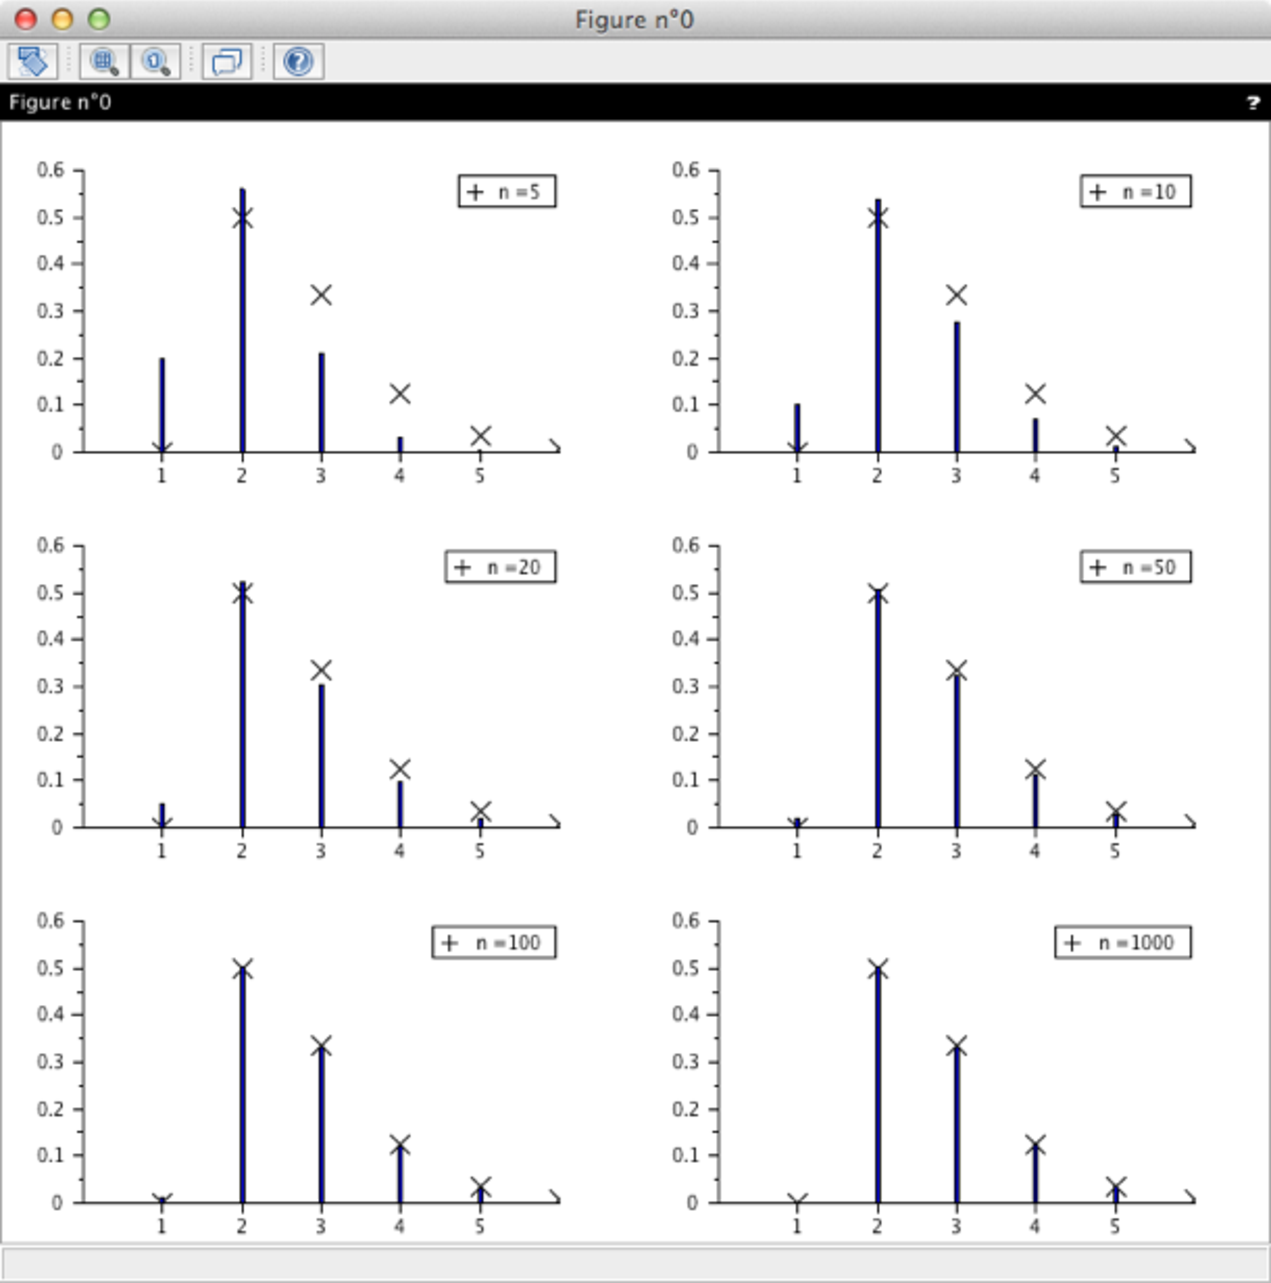
\includegraphics[height=13cm,width=13.13cm]
{Figures/Ecricome_2017/convergence_loi.pdf}
  \end{center}



  \begin{noliste}{a)}
  \item Expliquer ce que représentent les vecteurs renvoyés par les
    fonctions {\tt freqT} et {\tt loitheoY}. \\
    Comment ces vecteurs sont-ils représentés graphiquement dans
    chaque graphique obtenu ?
  
    \begin{proof}~\\
      Commençons par la description de la fonction {\tt loitheoY}.
      \begin{noliste}{$\sbullet$}
      \item La fonction {\tt loitheoY} renvoie un paramètre nommé {\tt
          y} qui est initialement affecté à un vecteur ligne de
        taille $n$ rempli de $0$ :\\[-.2cm]
        \begin{scilabC}{1}
          & \qquad \tcVar{y} = zeros(1,\tcVar{n}) \nl %
        \end{scilabC}
      \item Le $\eme{k}$ coefficient de ce vecteur est ensuite
        affecté à la valeur $\dfrac{k-1}{k!}$.
        \begin{scilabC}{3}
          & \qquad \qquad \tcVar{y}(k) = (k-1)/prod(1:k) \nl %
        \end{scilabC}
      \item On construit ainsi le vecteur : $\big( \Prob(\Ev{Y=1}),
        \Prob(\Ev{Y=2}), \ldots, \Prob(\Ev{Y={\tt n}}) \big)$.%
        \conc{L'instruction {\tt loitheoY(n)} renvoie un vecteur
          contenant la loi théorique de la \var $Y$.}
      \end{noliste}~\\%[.2cm]
      Traitons maintenant le cas de la fonction {\tt freqT}.
      \begin{noliste}{$\sbullet$}        
      \item Cette fonction renvoie un paramètre nommé {\tt y} qui est
        initialement affecté à un vecteur ligne de taille $n$ remplie
        de $0$ :\\[-.2cm]
        \begin{scilabC}{1}
          & \qquad \tcVar{y} = zeros(1,\tcVar{n}) \nl %
        \end{scilabC}
        
      \item La fonction a pour but de produire une approximation de la
        loi théorique de la \var $T_n$.\\
        On rappelle que $T_n(\Omega) = \llb 1, n \rrb$. La loi de
        $T_n$ est donc entièrement déterminée par les valeurs :
        \[
        \big(\Prob(\Ev{T_n = 1}), \Prob(\Ev{T_n = 2}), \ldots,
        \Prob(\Ev{T_n = n}) \big)
        \]
      \item Pour ce faire, l'idée est :
        \begin{noliste}{$\stimes$}
        \item de simuler un grand nombre de fois ($N = 100000$ est ce
          grand nombre) la \var $T_n$.\\
          Formellement, on souhaite obtenir un $N$-uplet $(z_1,
          \ldots, z_{N})$ qui correspond à l'observation d'un
          $N$-échantillon $(Z_1, \ldots, Z_{N})$ de la \var $T_n$.\\
          {\it (cela signifie que les \var $Z_1$, \ldots, $Z_{N}$ sont
            indépendantes et sont de même loi que $T_n$)}
        \item de compter le nombre de $1$, de $2$, \ldots, de $n$
          contenus dans cette observation.
        \end{noliste}
        Cette idée est justifiée par la loi faible des grands nombres
        (LfGN) qui affirme :
        \[
        \forall k \in \llb 1, n \rrb, \quad \dfrac{\text{nombre de $k$
            de l'observation}}{\text{taille ($N$) de l'observation}}
        \simeq \Prob(\Ev{T_n = k})
        \]
      \item Dans le programme, les valeurs $(z_1, \ldots, z_{N})$ sont
        obtenues par des appels successifs (à l'aide d'une structure
        itérative, ici une boucle \texttt{for}) à la fonction {\tt T}
        et stockées les unes après les autres dans la variable {\tt
          k}.
        \begin{scilabC}{2}
          & \quad \tcFor{for} i = 1 : 100000 \nl %
          & \quad \quad k = T(\tcVar{n}) \nl %
        \end{scilabC}
        Le tableau {\tt y} est alors mis à jour à chaque tour de
        boucle :
        \begin{scilabC}{4}
          & \quad \quad \tcVar{y}(k) = \tcVar{y}(k) + 1 \nl %
        \end{scilabC}


        \newpage


        \noindent
        Détaillons cette mise à jour : 
        \begin{noliste}{$\stimes$}
        \item \dashuline{si $\texttt{k}$ vaut $1$} alors
          l'instruction suivante est effectuée :
          \[
          \texttt{y(1) = y(1) + 1}
          \]
        \item \ldots
        \item \dashuline{si $\texttt{k}$ vaut $n$} alors l'instruction
          suivante est effectuée :
          \[
          \texttt{y(n) = y(n) + 1}
          \]
        \end{noliste}
        Cela signifie que le $\eme{k}$ coefficient du tableau
        compte le nombre de $k$ de l'observation.\\
        Une fois cette boucle effectuée, l'approximation formulée par
        la LfGN est obtenue en divisant ces nombres par la taille de
        l'observation :
        \begin{scilabC}{6}
          & \quad \tcVar{y} = \tcVar{y} / 100000 \nl %
        \end{scilabC}
      \item En résumé, l'instruction {\tt freqT(n)} renvoie un vecteur
        qui donne la fréquence d'apparition de chaque entier $k \in
        \llb 1, {\tt n} \rrb$ dans une observation de taille $100000$
        de la \var $T_n$. %
        \concL{D'après la LfGN, {\tt freqT(n)} renvoie un vecteur qui
          est une approximation du vecteur $\big(\Prob(\Ev{T_n = 1}),
          \Prob(\Ev{T_n = 2}), \ldots, \Prob(\Ev{T_n = n})
          \big)$.}{15.4}
      \end{noliste}
      
      
      
      % \newpage
      
      
      \noindent
      Commentons enfin la représentation graphique.
      \begin{noliste}{$\sbullet$}
      \item La ligne \ligne{10} du script permet de générer la
        représentation graphique du vecteur issu de la fonction {\tt
          loitheoY} :
        \begin{scilabC}{9}
          &  plot2d(loitheoY(6), style=-2) \nl %
        \end{scilabC}
        Rappelons que {\tt style=-2} est l'argument de la commande
        {\tt plot2d} permettant d'afficher les points dans le plan
        avec des croix.  %
        \conc{Le vecteur {\tt loitheoY(6)} est représenté
          graphiquement par des croix.}

      \item La ligne \ligne{10} du script permet de générer la
        représentation graphique du vecteur issu de la fonction {\tt
          freqT} :
        \begin{scilabC}{10}
          & x = freqT(n) \nl %
          & bar(x(1:5)) \nl %
        \end{scilabC}
        Rappelons que {\tt bar} est une commande générant un diagramme
        en bâtons.%
        \conc{Le vecteur {\tt x} issu de l'instruction {\tt x =
            freqT(n)} est représenté par un diagramme en bâtons.}
      \end{noliste}
      \begin{remark}%~\\
        \begin{noliste}{$\sbullet$}
        \item Il faut noter qu'on ne représente pas la loi de $Y$ en
          intégralité puisque l'appel {\tt loitheoY(6)} produit le
          vecteur : 
          \[
          \big( \Prob(\Ev{Y=1}), \Prob(\Ev{Y=2}), \ldots, \Prob(\Ev{Y=
            6}) \big)
          \]
          De même, l'instruction {\tt x(1:5)} sélectionne les $5$
          premiers coefficients du vecteur généré par {\tt x =
            freqT(n)}. On obtient ainsi une approximation du vecteur :
          \[
          \big( \Prob(\Ev{T_n = 1}), \Prob(\Ev{Y=2}), \ldots,
          \Prob(\Ev{T_n= 5}) \big)
          \]
          {\tt }
        \item Les croix sont placées exactement au même endroit sur
          les $6$ graphiques. C'est logique puisque le vecteur {\tt
            loitheoY(6)} est indépendant de la valeur prise par $n$.
        \end{noliste}
      \end{remark}~\\[-1.4cm]
    \end{proof}
    
    
    \newpage


  \item Expliquer en quoi cette succession de graphiques permet
    d'illustrer le résultat de la question \itbf{13}.
  
    \begin{proof}~
      \begin{noliste}{$\sbullet$}
      \item D'après la question précédente :
        \begin{noliste}{$\stimes$}
        \item le vecteur {\tt freqT(n)} est une approximation de la
          loi de $T_{\tt n}$.
        \item le vecteur {\tt loitheoY(n)} représente la loi de $Y$.
        \end{noliste}

      \item La succession de graphiques démontre que, lorsque la valeur
        de {\tt n} grandit, les coefficients de {\tt freqT(n)} se
        rapprochent de ceux de {\tt loitheoY(n)}. Dès la valeur {\tt
          n} $= 50$, les deux graphiques semblent très proches. Pour
        {\tt n} $= 1000$ les deux graphiques coïncident même à
        l'\oe{}il nu.

      \item Cette succession de graphiques illustre donc la propriété :
        \[
        \forall k \in \N^*, \quad \Prob(\Ev{T_n = k}) \tendn
        \Prob(\Ev{Y = k})
        \]
        (le $\eme{k}$ coefficient de {\tt freqT(n)} se rapproche du
        $\eme{k}$ coefficient de {\tt loitheoY(n)} lorsque l'entier
        {\tt n} grandit)
      \end{noliste}
      \conc{Cette succession de graphiques permet d'illustrer la
        convergence en loi de $(T_n)$ vers $Y$.}
      \begin{remark}%~\\
        \begin{noliste}{$\sbullet$}
        \item Cette succession de graphiques permet aussi de parler de
          vitesse de convergence. On s'aperçoit que l'approximation de
          {\tt loitheoY(n)} par {\tt freqT(n)} est déjà correcte pour
          {\tt n} $=10$; satisfaisante pour {\tt n} $=20$; bonne pour
          {\tt n} $=50$ et encore meilleure pour les valeurs
          suivantes. Ceci suggère que la \var $T_n$ converge en loi
          vers la \var $Y$ de manière très rapide.
        \item On a évoqué en question \itbf{15.} la loi faible des
          grands nombres (LfGN). L'idée est de simuler un grand nombre
          de fois ($N$ fois) la \var $T_n$ (à $n$ fixé) afin d'obtenir
          une répartition des valeurs possibles de $T_n$ et ainsi une
          approximation de la loi de $T_n$. Dans l'énoncé, on fait le
          choix $N = 100000$. Cela suggère que le résultat de
          convergence fournit par la LfGN a une vitesse de convergence
          faible : $N$ doit être un nombre réellement {\bf grand} pour
          que l'approximation obtenue soit bonne.
        \end{noliste}
      \end{remark}~\\[-1.4cm]
    \end{proof}    
  \end{noliste}
\end{noliste}


